\documentclass[]{article}
\usepackage{lmodern}
\usepackage{amssymb,amsmath}
\usepackage{ifxetex,ifluatex}
\usepackage{fixltx2e} % provides \textsubscript
\ifnum 0\ifxetex 1\fi\ifluatex 1\fi=0 % if pdftex
  \usepackage[T1]{fontenc}
  \usepackage[utf8]{inputenc}
\else % if luatex or xelatex
  \ifxetex
    \usepackage{mathspec}
  \else
    \usepackage{fontspec}
  \fi
  \defaultfontfeatures{Ligatures=TeX,Scale=MatchLowercase}
\fi
% use upquote if available, for straight quotes in verbatim environments
\IfFileExists{upquote.sty}{\usepackage{upquote}}{}
% use microtype if available
\IfFileExists{microtype.sty}{%
\usepackage{microtype}
\UseMicrotypeSet[protrusion]{basicmath} % disable protrusion for tt fonts
}{}
\usepackage[margin=1in]{geometry}
\usepackage{hyperref}
\hypersetup{unicode=true,
            pdftitle={The EMU-SDMS Manual},
            pdfauthor={Raphael Winkelmann},
            pdfborder={0 0 0},
            breaklinks=true}
\urlstyle{same}  % don't use monospace font for urls
\usepackage{natbib}
\bibliographystyle{plainnat}
\usepackage{color}
\usepackage{fancyvrb}
\newcommand{\VerbBar}{|}
\newcommand{\VERB}{\Verb[commandchars=\\\{\}]}
\DefineVerbatimEnvironment{Highlighting}{Verbatim}{commandchars=\\\{\}}
% Add ',fontsize=\small' for more characters per line
\usepackage{framed}
\definecolor{shadecolor}{RGB}{248,248,248}
\newenvironment{Shaded}{\begin{snugshade}}{\end{snugshade}}
\newcommand{\AlertTok}[1]{\textcolor[rgb]{0.94,0.16,0.16}{#1}}
\newcommand{\AnnotationTok}[1]{\textcolor[rgb]{0.56,0.35,0.01}{\textbf{\textit{#1}}}}
\newcommand{\AttributeTok}[1]{\textcolor[rgb]{0.77,0.63,0.00}{#1}}
\newcommand{\BaseNTok}[1]{\textcolor[rgb]{0.00,0.00,0.81}{#1}}
\newcommand{\BuiltInTok}[1]{#1}
\newcommand{\CharTok}[1]{\textcolor[rgb]{0.31,0.60,0.02}{#1}}
\newcommand{\CommentTok}[1]{\textcolor[rgb]{0.56,0.35,0.01}{\textit{#1}}}
\newcommand{\CommentVarTok}[1]{\textcolor[rgb]{0.56,0.35,0.01}{\textbf{\textit{#1}}}}
\newcommand{\ConstantTok}[1]{\textcolor[rgb]{0.00,0.00,0.00}{#1}}
\newcommand{\ControlFlowTok}[1]{\textcolor[rgb]{0.13,0.29,0.53}{\textbf{#1}}}
\newcommand{\DataTypeTok}[1]{\textcolor[rgb]{0.13,0.29,0.53}{#1}}
\newcommand{\DecValTok}[1]{\textcolor[rgb]{0.00,0.00,0.81}{#1}}
\newcommand{\DocumentationTok}[1]{\textcolor[rgb]{0.56,0.35,0.01}{\textbf{\textit{#1}}}}
\newcommand{\ErrorTok}[1]{\textcolor[rgb]{0.64,0.00,0.00}{\textbf{#1}}}
\newcommand{\ExtensionTok}[1]{#1}
\newcommand{\FloatTok}[1]{\textcolor[rgb]{0.00,0.00,0.81}{#1}}
\newcommand{\FunctionTok}[1]{\textcolor[rgb]{0.00,0.00,0.00}{#1}}
\newcommand{\ImportTok}[1]{#1}
\newcommand{\InformationTok}[1]{\textcolor[rgb]{0.56,0.35,0.01}{\textbf{\textit{#1}}}}
\newcommand{\KeywordTok}[1]{\textcolor[rgb]{0.13,0.29,0.53}{\textbf{#1}}}
\newcommand{\NormalTok}[1]{#1}
\newcommand{\OperatorTok}[1]{\textcolor[rgb]{0.81,0.36,0.00}{\textbf{#1}}}
\newcommand{\OtherTok}[1]{\textcolor[rgb]{0.56,0.35,0.01}{#1}}
\newcommand{\PreprocessorTok}[1]{\textcolor[rgb]{0.56,0.35,0.01}{\textit{#1}}}
\newcommand{\RegionMarkerTok}[1]{#1}
\newcommand{\SpecialCharTok}[1]{\textcolor[rgb]{0.00,0.00,0.00}{#1}}
\newcommand{\SpecialStringTok}[1]{\textcolor[rgb]{0.31,0.60,0.02}{#1}}
\newcommand{\StringTok}[1]{\textcolor[rgb]{0.31,0.60,0.02}{#1}}
\newcommand{\VariableTok}[1]{\textcolor[rgb]{0.00,0.00,0.00}{#1}}
\newcommand{\VerbatimStringTok}[1]{\textcolor[rgb]{0.31,0.60,0.02}{#1}}
\newcommand{\WarningTok}[1]{\textcolor[rgb]{0.56,0.35,0.01}{\textbf{\textit{#1}}}}
\usepackage{longtable,booktabs}
\usepackage{graphicx,grffile}
\makeatletter
\def\maxwidth{\ifdim\Gin@nat@width>\linewidth\linewidth\else\Gin@nat@width\fi}
\def\maxheight{\ifdim\Gin@nat@height>\textheight\textheight\else\Gin@nat@height\fi}
\makeatother
% Scale images if necessary, so that they will not overflow the page
% margins by default, and it is still possible to overwrite the defaults
% using explicit options in \includegraphics[width, height, ...]{}
\setkeys{Gin}{width=\maxwidth,height=\maxheight,keepaspectratio}
\IfFileExists{parskip.sty}{%
\usepackage{parskip}
}{% else
\setlength{\parindent}{0pt}
\setlength{\parskip}{6pt plus 2pt minus 1pt}
}
\setlength{\emergencystretch}{3em}  % prevent overfull lines
\providecommand{\tightlist}{%
  \setlength{\itemsep}{0pt}\setlength{\parskip}{0pt}}
\setcounter{secnumdepth}{5}
% Redefines (sub)paragraphs to behave more like sections
\ifx\paragraph\undefined\else
\let\oldparagraph\paragraph
\renewcommand{\paragraph}[1]{\oldparagraph{#1}\mbox{}}
\fi
\ifx\subparagraph\undefined\else
\let\oldsubparagraph\subparagraph
\renewcommand{\subparagraph}[1]{\oldsubparagraph{#1}\mbox{}}
\fi

%%% Use protect on footnotes to avoid problems with footnotes in titles
\let\rmarkdownfootnote\footnote%
\def\footnote{\protect\rmarkdownfootnote}

%%% Change title format to be more compact
\usepackage{titling}

% Create subtitle command for use in maketitle
\newcommand{\subtitle}[1]{
  \posttitle{
    \begin{center}\large#1\end{center}
    }
}

\setlength{\droptitle}{-2em}
  \title{The EMU-SDMS Manual}
  \pretitle{\vspace{\droptitle}\centering\huge}
  \posttitle{\par}
  \author{Raphael Winkelmann}
  \preauthor{\centering\large\emph}
  \postauthor{\par}
  \date{}
  \predate{}\postdate{}

\usepackage{booktabs}
\usepackage{amsthm}
\makeatletter
\def\thm@space@setup{%
  \thm@preskip=8pt plus 2pt minus 4pt
  \thm@postskip=\thm@preskip
}
\makeatother

\usepackage{amsthm}
\newtheorem{theorem}{Theorem}[section]
\newtheorem{lemma}{Lemma}[section]
\theoremstyle{definition}
\newtheorem{definition}{Definition}[section]
\newtheorem{corollary}{Corollary}[section]
\newtheorem{proposition}{Proposition}[section]
\theoremstyle{definition}
\newtheorem{example}{Example}[section]
\theoremstyle{definition}
\newtheorem{exercise}{Exercise}[section]
\theoremstyle{remark}
\newtheorem*{remark}{Remark}
\newtheorem*{solution}{Solution}
\begin{document}
\maketitle

{
\setcounter{tocdepth}{2}
\tableofcontents
}
\hypertarget{welcome}{%
\section*{Welcome}\label{welcome}}
\addcontentsline{toc}{section}{Welcome}

\begin{center}
\includegraphics[width=0.35\linewidth]{pics/EMU-webAppIcon-roundCorners} \end{center}

Welcome to the EMU-SDMS Manual!

{ Disclaimer: This manual is still in the making! It will eventually
replace all the vignettes of emuR, wrassp as well as the EMU-webApp's
own documentation. This manual is intended to consolidate all of this
information in one easy to find location that can easily be updated as
new features are added.}

\hypertarget{installing-the-emu-sdms}{%
\section{Installing the EMU-SDMS}\label{installing-the-emu-sdms}}

\begin{enumerate}
\def\labelenumi{\arabic{enumi}.}
\tightlist
\item
  R

  \begin{itemize}
  \tightlist
  \item
    Download the R programming language from
    \url{https://cran.r-project.org/}
  \item
    Install the R programming language by executing the downloaded file
    and following the on-screen instructions.
  \end{itemize}
\item
  \texttt{emuR}

  \begin{itemize}
  \tightlist
  \item
    Start up R.
  \item
    Enter \texttt{install.packages("emuR")} after the
    \texttt{\textgreater{}} prompt to install the package. (You will
    only need to repeat this if package updates become available.)
  \item
    As the \texttt{wrassp} package is a dependency of the \texttt{emuR}
    package, it does not have to be installed separately.
  \end{itemize}
\item
  \texttt{EMU-webApp} (prerequisite)

  \begin{itemize}
  \tightlist
  \item
    The only thing needed to use the \texttt{EMU-webApp} is a current
    HTML5 compatible browser (Chrome/Firefox/Safari/Opera/\ldots{}).
    However, as most of the development and testing is done using Chrome
    we recommend using it, as it is by far the best tested browser.
  \end{itemize}
\end{enumerate}

\hypertarget{version-disclaimer}{%
\subsection{Version disclaimer}\label{version-disclaimer}}

This document describes the following versions of the software
components:

\begin{itemize}
\tightlist
\item
  \texttt{wrassp}

  \begin{itemize}
  \tightlist
  \item
    Package version: 0.1.6
  \item
    Git tag name: v0.1.6 (on master branch)
  \end{itemize}
\item
  \texttt{emuR}

  \begin{itemize}
  \tightlist
  \item
    Package version: 1.0.0
  \item
    Git tag name: v1.0.0 (on master branch)
  \end{itemize}
\item
  \texttt{EMU-webApp}

  \begin{itemize}
  \tightlist
  \item
    Version: 0.1.12
  \item
    Git SHA1: 7b044a9f9fe19f2eb6d03ec6ec3f20d5b1d25db2
  \end{itemize}
\end{itemize}

As the development of the EMU Speech Database Management System is still
ongoing, be sure you have the correct documentation to go with the
version you are using.

\hypertarget{for-developers-and-people-interested-in-the-source-code}{%
\subsection{For developers and people interested in the source
code}\label{for-developers-and-people-interested-in-the-source-code}}

The information on how to install and/or access the source code of the
developer version including the possibility of accessing the versions
described in this document (via the Git tag names mentioned above) is
given below.

\begin{itemize}
\tightlist
\item
  \texttt{wrassp}

  \begin{itemize}
  \tightlist
  \item
    Source code is available here:
    \url{https://github.com/IPS-LMU/wrassp/}
  \item
    Install developer version in R:
    \texttt{install.packages("devtools");} \texttt{library("devtools");}
    \texttt{install\_github("IPS-LMU/wrassp")}
  \item
    Bug reports: \url{https://github.com/IPS-LMU/wrassp/issues}
  \end{itemize}
\item
  \texttt{emuR}

  \begin{itemize}
  \tightlist
  \item
    Source code is available here:
    \url{https://github.com/IPS-LMU/emuR/}
  \item
    Install developer version in R:
    \texttt{install.packages("devtools");} \texttt{library("devtools");}
    \texttt{install\_github("IPS-LMU/emuR")}
  \item
    Bug reports: \url{https://github.com/IPS-LMU/emuR/issues}
  \end{itemize}
\item
  \texttt{EMU-webApp}

  \begin{itemize}
  \tightlist
  \item
    Source code is available here:
    \url{https://github.com/IPS-LMU/EMU-webApp/}
  \item
    Bug reports: \url{https://github.com/IPS-LMU/EMU-webApp/issues}
  \end{itemize}
\end{itemize}

\hypertarget{part-overview-and-tutorial}{%
\part{Overview and
tutorial}\label{part-overview-and-tutorial}}

\hypertarget{chap:overview}{%
\section[An overview of the EMU-SDMS ]{\texorpdfstring{An overview of
the EMU-SDMS \footnote{Sections of this chapter have been published in
  \citet{winkelmann:2017aa}}}{An overview of the EMU-SDMS }}\label{chap:overview}}

\begin{center}
\includegraphics[width=0.35\linewidth]{pics/EMU-webAppIcon-roundCorners} \end{center}

The EMU Speech Database Management System (EMU-SDMS) is a collection of
software tools which aims to be as close to an all-in-one solution for
generating, manipulating, querying, analyzing and managing speech
databases as possible. It was developed to fill the void in the
landscape of software tools for the speech sciences by providing an
integrated system that is centered around the R language and environment
for statistical computing and graphics (\citet{r-core-team:2016a}). This
manual contains the documentation for the three software components
\texttt{wrassp}, \texttt{emuR} and the \texttt{EMU-webApp}. In addition,
it provides an in-depth description of the \texttt{emuDB} database
format which is also considered an integral part of the new system.
These four components comprise the EMU-SDMS and benefit the speech
sciences and spoken language research by providing an integrated system
to answer research questions such as: \emph{Given an annotated speech
database, is the vowel height of the vowel @ (measured by its correlate,
the first formant frequency) influenced by whether it appears in a
strong or weak syllable?}

This manual is targeted at new EMU-SDMS users as well as users familiar
with the legacy EMU system. In addition, it is aimed at people who are
interested in the technical details such as data structures/formats and
implementation strategies, be it for reimplementation purposes or simply
for a better understanding of the inner workings of the new system. To
accommodate these different target groups, after initially giving an
overview of the system, this manual presents a usage tutorial that walks
the user through the entire process of answering a research question.
This tutorial will start with a set of \texttt{.wav} audio and Praat
\texttt{.TextGrid} (\citet{boersma:2011a}) annotation files and end with
a statistical analysis to address the hypothesis posed by the research
question. The following Part \ref{part:mainCompAndConc} of this
documentation is separated into six chapters that give an in-depth
explanation of the various components that comprise the EMU-SDMS and
integral concepts of the new system. These chapters provide a
tutorial-like overview by providing multiple examples. To give the
reader a synopsis of the main functions and central objects that are
provided by EMU-SDMS's main R package \texttt{emuR}, an overview of
these functions is presented in Part \ref{part:emuRfuncs}. Part
\ref{part:impl} focuses on the actual implementation of the components
and is geared towards people interested in the technical details.
Further examples and file format descriptions are available in various
appendices. This structure enables the novice EMU-SDMS user to simply
skip the technical details and still get an in-depth overview of how to
work with the new system and discover what it is capable of.

A prerequisite that is presumed throughout this document is the reader's
familiarity with basic terminology in the speech sciences (e.g.,
familiarity with the international phonetic alphabet (IPA) and how
speech is annotated at a coarse and fine grained level). Further, we
assume the reader has a grasp of the basic concepts of the R language
and environment for statistical computing and graphics. For readers new
to R, there are multiple, freely available R tutorials online (e.g.,
\url{https://en.wikibooks.org/wiki/Statistical_Analysis:_an_Introduction_using_R/R_basics}).
R also has a set of very detailed manuals and tutorials that come
preinstalled with R. To be able to access R's own ``An Introduction to
R'' introduction, simply type \texttt{help.start()} into the R console
and click on the link to the tutorial.

\hypertarget{the-evolution-of-the-emu-sdms}{%
\subsection{The evolution of the
EMU-SDMS}\label{the-evolution-of-the-emu-sdms}}

The EMU-SDMS has a number of predecessors that have been continuously
developed over a number of years (e.g., \citet{harrington:csl1993a},
\citet{cassidy:1996a}, \citet{cassidy:sc2001a}, \citet{bombien:2006a},
\citet{harrington:2010a}, \citet{john:2012a}). The components presented
here are the completely rewritten and newly designed, next incarnation
of the EMU system, which we will refer to as the EMU Speech Database
Management System (EMU-SDMS). The EMU-SDMS keeps most of the core
concepts of the previous system, which we will refer to as the legacy
system, in place while improving on things like usability,
maintainability, scalability, stability, speed and more. We feel the
redesign and reimplementation elevates the system into a modern set of
speech and language tools that enables a workflow adapted to the
challenges confronting speech scientists and the ever growing size of
speech databases. The redesign has enabled us to implement several
components of the new EMU-SDMS so that they can be used independently of
the EMU-SDMS for tasks such as web-based collaborative annotation
efforts and performing speech signal processing in a statistical
programming environment. Nevertheless, the main goal of the redesign and
reimplementation was to provide a modern set of tools that reduces the
complexity of the tool chain needed to answer spoken language research
questions down to a few interoperable tools. The tools the EMU-SDMS
provides are designed to streamline the process of obtaining usable
data, all from within an environment that can also be used to analyze,
visualize and statistically evaluate the data.

Upon developing the new system, rather than starting completely from
scratch it seemed more appropriate to partially reuse the concepts of
the legacy system in order to achieve our goals. A major observation at
the time was that the R language and environment for statistical
computing and graphics (\citet{r-core-team:2016a}) was gaining more and
more traction for statistical and data visualization purposes in the
speech and spoken language research community. However, R was mostly
only used towards the end of the data analysis chain where data usually
was pre-converted into a comma-separated values or equivalent file
format by the user using other tools to calculate, extract and
pre-process the data. While designing the new EMU-SDMS, we brought R to
the front of the tool chain to the point just beyond data acquisition.
This allows the entire data annotation, data extraction and analysis
process to be completed in R, while keeping the key user requirements in
mind. Due to personal experiences gained by using the legacy system for
research puposes and in various undergraduate courses (course material
usually based on \citet{harrington:2010a}), we learned that the key user
requirements were data and database portability, a simple installation
process, a simplified/streamlined user experience and cross-platform
availability. Supplying all of EMU-SDMS's core functionality in the form
of R packages that do not rely on external software at runtime seemed to
meet all of these requirements.

As the early incarnations of the legacy EMU system and its predecessors
were conceived either at a time that predated the R system or during the
infancy of R's package ecosystem, the legacy system was implemented as a
modular yet composite standalone program with a communication and data
exchange interface to the R/Splus systems (see \citet{cassidy:sc2001a}
Section 3 for details). Recent developments in the package ecosystem of
R such as the availability of the \texttt{DBI} package
(\citet{r-special-interest-group-on-databases-r-sig-db:2016a}) and the
related packages \texttt{RSQLite} and \texttt{RPostgreSQL}
(\citet{wickham:2014a}, \citet{conway:2016a}), as well as the
\texttt{jsonlite} package (\citet{ooms:as2014a}) and the \texttt{httpuv}
package (\citet{rstudio:2015a}), have made R an attractive sole target
platform for the EMU-SDMS. These and other packages provide additional
functional power that enabled the EMU-SDMS's core functionality to be
implemented in the form of R packages. The availability of certain R
packages had a large impact on the architectural design decisions that
we made for the new system.

R Example \ref{rexample:overview-install} shows the simple installation
process which we were able to achieve due to the R package
infrastructure. Compared to the legacy EMU and other systems, the
installation process of the entire system has been reduced to a single R
command. Throughout this documentation we will try to highlight how the
EMU-SDMS is also able to meet the rest of the above key user
requirements.

rexample:overview-install

\begin{Shaded}
\begin{Highlighting}[]
\CommentTok{# install the entire EMU-SDMS}
\CommentTok{# by installing the emuR package}
\KeywordTok{install.packages}\NormalTok{(}\StringTok{"emuR"}\NormalTok{)}
\end{Highlighting}
\end{Shaded}

It is worth noting that throughout this manual R Example code snippets
will be given in the form of R Example \ref{rexample:overview-install}.
These examples represent working R code that allow the reader to follow
along in a hands-on manor and give a feel for what it is like working
with the new EMU-SDMS.

\hypertarget{sec:overview-sysArch}{%
\subsection{EMU-SDMS: System architecture and default
workflow}\label{sec:overview-sysArch}}

As was previously mentioned, the new EMU-SDMS is made up of four main
components. The components are the \texttt{emuDB} format; the R packages
\texttt{wrassp} and \texttt{emuR}; and the web application, the
\texttt{EMU-webApp}, which is EMU-SDMS's new GUI component. An overview
of the EMU-SDMS's architecture and the components' relationships within
the system is shown in Figure \ref{fig:overview-archOver}. In Figure
\ref{fig:overview-archOver}, the \texttt{emuR} package plays a central
role as it is the only component that interacts with all of the other
components of the EMU-SDMS. It performs file and DB handling for the
files that comprise an \texttt{emuDB} (see Chapter
@ref(chap:annot\_struct\_mod)); it uses the \texttt{wrassp} package for
signal processing purposes (see Chapter \ref{chap:wrassp}; and it can
serve \texttt{emuDB}s to the \texttt{EMU-webApp} (see Chapter
\ref{chap:emu-webApp}).

\begin{figure}

{\centering 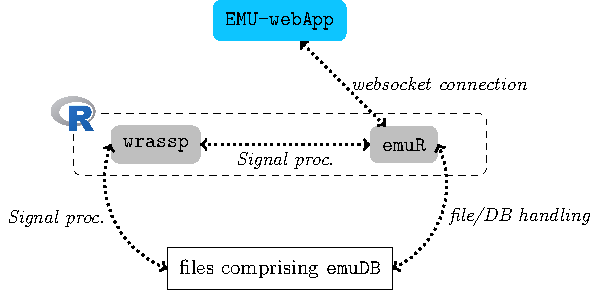
\includegraphics[width=0.75\linewidth]{pics/overview} 

}

\caption{Schematic architecture of the EMU-SDMS}\label{fig:overview-archOver}
\end{figure}

Although the system is made of four main components, the user largely
only interacts directly with the \texttt{EMU-webApp} and the
\texttt{emuR} package. A summary of the default workflow illustrating
theses interactions can be seen below:

\begin{enumerate}
\def\labelenumi{\arabic{enumi}.}
\tightlist
\item
  Load database into current R session (\texttt{load\_emuDB()}).
\item
  Database annotation / visual inspection (\texttt{serve()}). This opens
  up the \texttt{EMU-webApp} in the system's default browser.
\item
  Query database (\texttt{query()}). This is optionally followed by
  \texttt{requery\_hier()} or \texttt{requery\_seq()} as necessary (see
  Chapter \ref{chap:querysys} for details).
\item
  Get trackdata (e.g.~formant values) for the result of a query
  (\texttt{get\_trackdata()}).
\item
  Prepare data.
\item
  Visually inspect data.
\item
  Carry out further analysis and statistical processing.
\end{enumerate}

Initially the user creates a reference to an \texttt{emuDB} by loading
it into their current R session using the \texttt{load\_emuDB()}
function (see step 1). This database reference can then be used to
either serve (\texttt{serve()}) the database to the \texttt{EMU-webApp}
or query (\texttt{query()}) the annotations of the \texttt{emuDB} (see
steps 2 and 3). The result of a query can then be used to either perform
one or more so-called requeries or extract signal values that correspond
to the result of a \texttt{query()} or \texttt{requery()} (see step 4).
Finally, the signal data can undergo further preparation (e.g.,
correction of outliers) and visual inspection before further analysis
and statistical processing is carried out (see steps 5, 6 and 7).
Although the R packages provided by the EMU-SDMS do provide functions
for steps 4, 5 and 6, it is worth noting that the plethora of R packages
that the R package ecosystem provides can and should be used to perform
these duties. The resulting objects of most of the above functions are
derived \texttt{matrix} or \texttt{data.frame} objects which can be used
as inputs for hundreds if not thousands of other R functions.

\hypertarget{emu-sdms-is-it-something-for-you}{%
\subsection{EMU-SDMS: Is it something for
you?}\label{emu-sdms-is-it-something-for-you}}

Besides providing a fully integrated system, the EMU-SDMS has several
unique features that set it apart from other current, widely used
systems (e.g., \citet{boersma:2011a}, \citet{wittenburg:2006a},
\citet{fromont:2012a}, \citet{rose:2006a}, \citet{mcauliffe:2016a}). To
our knowledge, the EMU-SDMS is the only system that allows the user to
model their annotation structures based on a hybrid model of time-based
annotations (such as those offered by Praat's tier-based annotation
mechanics) and hierarchical timeless annotations. An example of such a
hybrid annotation structure is displayed in Figure
\ref{fig:overview-hybridAnnot}. These hybrid annotations benefit the
user in multiple ways, as they reduce data redundancy and explicitly
allow relationships to be expressed across annotation levels (see
Chapter \ref{chap:annot_struct_mod} for further information on
hierarchical annotations and Chapter \ref{chap:querysys} on how to query
these annotation structures).

\begin{figure}

{\centering 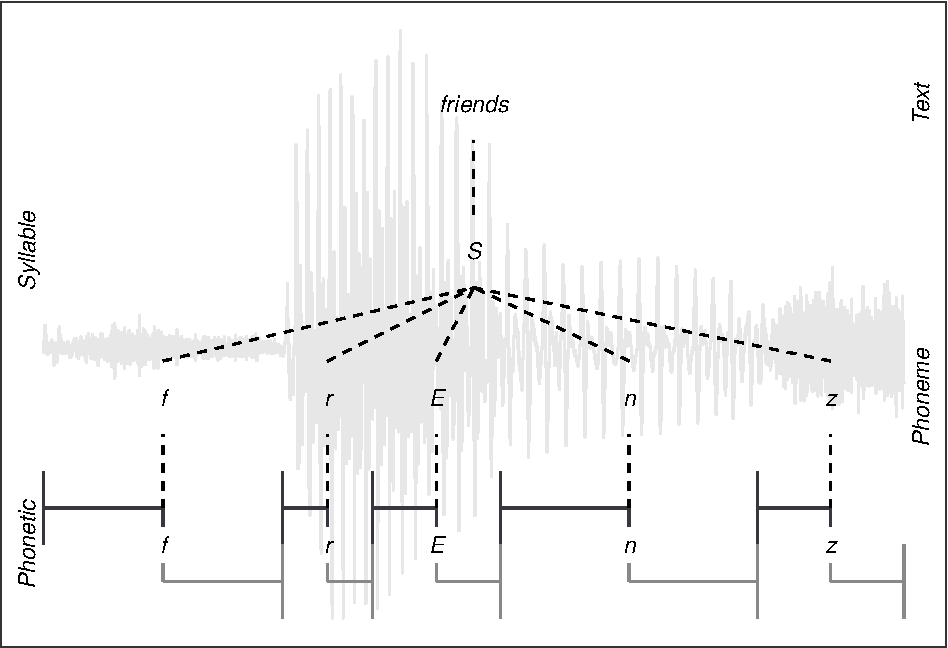
\includegraphics[width=0.75\linewidth]{overview_files/figure-latex/overview-hybridAnnot-1} 

}

\caption{Example of a hybrid annotation combining time-based (*Phonetic* level) and hierarchical (*Phoneme*, *Syllable*, *Text* levels including the inter-level links) annotations.}\label{fig:overview-hybridAnnot}
\end{figure}

Further, to our knowledge, the EMU-SDMS is the first system that makes
use of a web application as its primary GUI for annotating speech. This
unique approach enables the GUI component to be used in multiple ways.
It can be used as a stand-alone annotation tool, connected to a loaded
\texttt{emuDB} via \texttt{emuR}'s \texttt{serve()} function and used to
communicate to other servers. This enables it to be used as a
collaborative annotation tool. An in-depth explanation of how this
component can be used in these three scenarios is given in Chapter
\ref{chap:emu-webApp}.

As demonstrated in the default workflow of Section
\ref{sec:overview-sysArch}, an additional unique feature provided by
EMU-SDMS is the ability to use the result of a query to extract derived
(e.g., formants and RMS values) and complementary signals (e.g.,
electromagnetic articulography (EMA) data) that match the segments of a
query. This, for example, aids the user in answering questions related
to derived speech signals such as: \emph{Is the vowel height of the
vowel @ (measured by its correlate, the first formant frequency)
influenced by whether it appears in a strong or weak syllable?}. Chapter
\ref{chap:tutorial} gives a complete walk-through of how to go about
answering this question using the tools provided by the EMU-SDMS.

The features provided by the EMU-SDMS make it an all-in-one speech
database management solution that is centered around R. It enriches the
R platform by providing specialized speech signal processing, speech
database management, data extraction and speech annotation capabilities.
By achieving this without relying on any external software sources
except the web browser, the EMU-SDMS significantly reduces the number of
tools the speech and spoken language researcher has to deal with and
helps to simplify answering research questions. As the only prerequisite
for using the EMU-SDMS is a basic familiarity with the R platform, if
the above features would improve your workflow, the EMU-SDMS is indeed
for you.

\hypertarget{chap:tutorial}{%
\section[A tutorial on how to use the EMU-SDMS ]{\texorpdfstring{A
tutorial on how to use the EMU-SDMS \footnote{Some examples of this
  chapter are adapted versions of examples of the \texttt{emuR\_intro}
  vignette.}}{A tutorial on how to use the EMU-SDMS }}\label{chap:tutorial}}

\begin{center}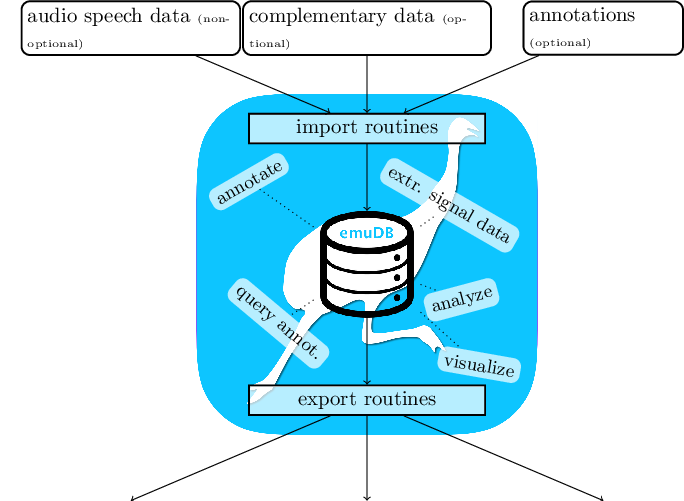
\includegraphics[width=0.65\linewidth]{pics/emuSdmsBirdsEye} \end{center}

Using the tools provided by the EMU-SDMS, this tutorial chapter gives a
practical step-by-step guide to answering the question: \emph{Given an
annotated speech database, is the vowel height of the vowel @ (measured
by its correlate, the first formant frequency) influenced by whether it
appears in a content or function word?} The tutorial only skims over
many of the concepts and functions provided by the EMU-SDMS. In-depth
explanations of the various functionalities are given in later chapters
of this documentation.

As the EMU-SDMS is not concerned with the raw data acquisition, other
tools such as SpeechRecorder by \citet{draxler:2004a} are first used to
record speech. However, once audio speech recordings are available, the
system provides multiple conversion routines for converting existing
collections of files to the new \texttt{emuDB} format described in
Chapter \ref{chap:emuDB} and importing them into the new EMU system. The
current import routines provided by the \texttt{emuR} package are:

\begin{itemize}
\tightlist
\item
  \texttt{convert\_TextGridCollection()} - Convert TextGrid collections
  (\texttt{.wav} and \texttt{.TextGrid} files) to the \texttt{emuDB}
  format,
\item
  \texttt{convert\_BPFCollection()} - Convert Bas Partitur Format (BPF)
  collections (\texttt{.wav} and \texttt{.par} files) to the
  \texttt{emuDB} format,
\item
  \texttt{convert\_txtCollection()} - Convert plain text file
  collections format (\texttt{.wav} and \texttt{.txt} files) to the
  \texttt{emuDB} format,
\item
  \texttt{convert\_legacyEmuDB()} - Convert the legacy EMU database
  format to the \texttt{emuDB} format and
\item
  \texttt{create\_emuDB()} followed by
  \texttt{add\_link/levelDefinition} and \texttt{import\_mediaFiles()} -
  Creating \texttt{emuDB}s from scratch with only audio files present.
\end{itemize}

The \texttt{emuR} package comes with a set of example files and small
databases that are used throughout the \texttt{emuR} documentation,
including the functions help pages. These can be accessed by typing
\texttt{help(functionName)} or the short form \texttt{?functionName}. R
Example \ref{rexample:tutorial-create-emuRdemoData} illustrates how to
create this demo data in a user-specified directory. Throughout the
examples of this documentation the directory that is provided by the
base R function \texttt{tempdir()} will be used, as this is available on
every platform supported by R (see \texttt{?tempdir} for further
details). As can be inferred from the \texttt{list.dirs()} output in R
Example \ref{rexample:tutorial-create-emuRdemoData}, the
\texttt{emuR\_demoData} directory contains a separate directory
containing example data for each of the import routines. Additionally,
it contains a directory containing an \texttt{emuDB} called \emph{ae}
(the directories name is \texttt{ae\_emuDB}, where \texttt{\_emuDB} is
the default suffix given to directories containing a \texttt{emuDB}; see
Chapter \ref{chap:emuDB}).

rexample:tutorial-create-emuRdemoData

\begin{Shaded}
\begin{Highlighting}[]
\CommentTok{# load the package}
\KeywordTok{library}\NormalTok{(emuR)}

\CommentTok{# create demo data in directory provided by the tempdir() function}
\CommentTok{# (of course other directory paths may be chosen)}
\KeywordTok{create_emuRdemoData}\NormalTok{(}\DataTypeTok{dir =} \KeywordTok{tempdir}\NormalTok{())}

\CommentTok{# create path to demo data directory, which is}
\CommentTok{# called "emuR_demoData"}
\NormalTok{demoDataDir =}\StringTok{ }\KeywordTok{file.path}\NormalTok{(}\KeywordTok{tempdir}\NormalTok{(), }\StringTok{"emuR_demoData"}\NormalTok{)}

\CommentTok{# show demo data directories}
\KeywordTok{list.dirs}\NormalTok{(demoDataDir, }\DataTypeTok{recursive =}\NormalTok{ F, }\DataTypeTok{full.names =}\NormalTok{ F)}
\end{Highlighting}
\end{Shaded}

\begin{verbatim}
## [1] "ae_emuDB"            "BPF_collection"      "legacy_ae"          
## [4] "TextGrid_collection" "txt_collection"
\end{verbatim}

This tutorial will start by converting a TextGrid collection containing
seven annotated single-sentence utterances of a single male speaker to
the \texttt{emuDB} format\footnote{The other input routines are covered
  in the Section @ref(sec:emuRpackageDetails\_importRoutines).}. In the
EMU-SDMS, a file collection such as a TextGrid collection refers to a
set of file pairs where two types of files with different file
extentions are present (e.g., \texttt{.ext1} and \texttt{.ext2}). It is
vital that file pairs have the same basenames (e.g., \texttt{A.ext1} and
\texttt{A.ext2} where \texttt{A} represents the basename) in order for
the conversion functions to be able to pair up files that belong
together. As other speech software tools also encourage such file pairs
(e.g., \citet{kisler:2015a}) this is a common collection format in the
speech sciences. R Example \ref{rexample:showTGcolContent} shows such a
file collection that is part of \texttt{emuR}'s demo data. Figure
@ref(fig:msajc003\_praatTG) shows the content of an annotation as
displayed by Praat's \texttt{"Draw\ visible\ sound\ and\ Textgrid..."}
procedure.

rexample:showTGcolContent

\begin{Shaded}
\begin{Highlighting}[]
\CommentTok{# create path to TextGrid collection}
\NormalTok{tgColDir =}\StringTok{ }\KeywordTok{file.path}\NormalTok{(demoDataDir, }\StringTok{"TextGrid_collection"}\NormalTok{)}

\CommentTok{# show content of TextGrid_collection directory}
\KeywordTok{list.files}\NormalTok{(tgColDir)}
\end{Highlighting}
\end{Shaded}

\begin{verbatim}
##  [1] "msajc003.TextGrid" "msajc003.wav"      "msajc010.TextGrid"
##  [4] "msajc010.wav"      "msajc012.TextGrid" "msajc012.wav"     
##  [7] "msajc015.TextGrid" "msajc015.wav"      "msajc022.TextGrid"
## [10] "msajc022.wav"      "msajc023.TextGrid" "msajc023.wav"     
## [13] "msajc057.TextGrid" "msajc057.wav"
\end{verbatim}

\textbackslash{}begin\{figure\}

\{\centering 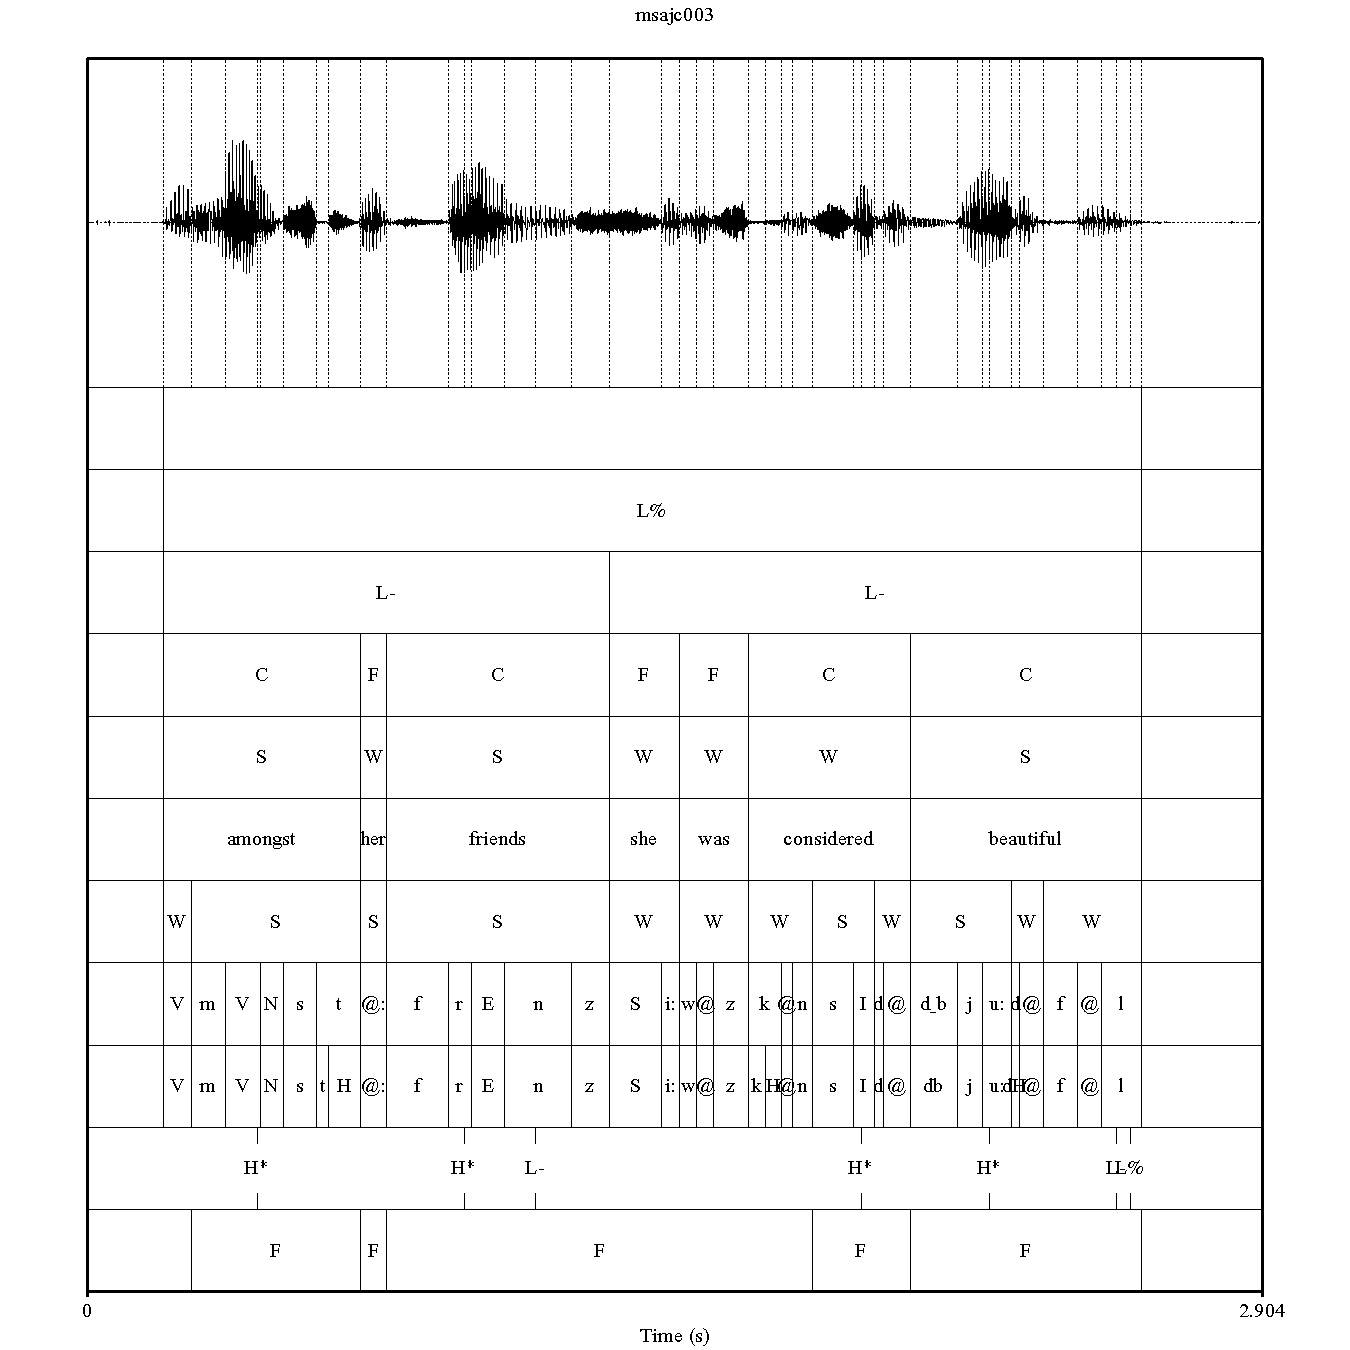
\includegraphics[width=0.85\linewidth]{pics/msajc003_praat}

\}

\textbackslash{}caption\{TextGrid annotation of the
\texttt{emuR\_demoData/TextGrid\_collection/msajc003.wav} /
\texttt{.TextGrid} file pair containing the tiers (from top to bottom):
\emph{Utterance}, \emph{Intonational}, \emph{Intermediate}, \emph{Word},
\emph{Accent}, \emph{Text}, \emph{Syllable}, \emph{Phoneme},
\emph{Phonetic}, \emph{Tone}, \emph{Foot}.\}(\#fig:msajc003\_praatTG)
\textbackslash{}end\{figure\}

\hypertarget{converting-the-textgrid-collection}{%
\subsection{Converting the TextGrid
collection}\label{converting-the-textgrid-collection}}

The \texttt{convert\_TextGridCollection()} function converts a TextGrid
collection to the \texttt{emuDB} format. A precondition that all
\texttt{.TextGrid} files have to fulfill is that they must all contain
the same tiers. If this is not the case, yet there is an equal tier
subset that is contained in all the TextGrid files, this equal subset
may be chosen. For example, if all \texttt{.TextGrid} files contain only
the tier \texttt{Phonetic:\ IntervalTier} the conversion will work.
However, if a single \texttt{.TextGrid} of the collection has the
additional tier \texttt{Tone:\ TextTier} the conversion will fail. In
this case the conversion could be made to work by specifying the equal
subset (e.g., \texttt{equalSubset\ =\ c("Phonetic")}) and passing it on
to the \texttt{tierNames} function argument
\texttt{convert\_TextGridCollection(...,\ tierNames\ =\ equalSubset,\ ...)}.
As can be seen in Figure \ref{fig:msajc003-praatTG}, the TextGrid files
provided by the demo data contain eleven tiers. To reduce the complexity
of the annotations for this tutorial we will only convert the tiers
\emph{Word} (content: \emph{C} vs.~function: \emph{F} word annotations),
\emph{Syllable} (strong: \emph{S} vs.~weak: \emph{W} syllable
annotations), \emph{Phoneme} (phoneme level annotations) and
\emph{Phonetic} (phonetic annotations using Speech Assessment Methods
Phonetic Alphabet (SAMPA) symbols - \citet{wells:1997aa}) using the
\texttt{tierNames} parameter. This conversion can be seen in R Example
@ref(rexample:tutorial\_tgconv).

rexample:tutorial\_tgconv

\begin{Shaded}
\begin{Highlighting}[]
\CommentTok{# convert TextGrid collection to the emuDB format}
\KeywordTok{convert_TextGridCollection}\NormalTok{(}\DataTypeTok{dir =}\NormalTok{ tgColDir,}
                           \DataTypeTok{dbName =} \StringTok{"myFirst"}\NormalTok{,}
                           \DataTypeTok{targetDir =} \KeywordTok{tempdir}\NormalTok{(),}
                           \DataTypeTok{tierNames =} \KeywordTok{c}\NormalTok{(}\StringTok{"Word"}\NormalTok{, }\StringTok{"Syllable"}\NormalTok{,}
                                         \StringTok{"Phoneme"}\NormalTok{, }\StringTok{"Phonetic"}\NormalTok{))}
\end{Highlighting}
\end{Shaded}

The above call to \texttt{convert\_TextGridCollection()} creates a new
\texttt{emuDB} directory in the \texttt{tempdir()} directory called
\texttt{myFirst\_emuDB}. This \texttt{emuDB} contains annotation files
that contain the same \emph{Word}, \emph{Syllable}, \emph{Phoneme} and
\emph{Phonetic} segment tiers as the original \texttt{.TextGrid} files
as well as copies of the original (\texttt{.wav}) audio files. For
further details about the structure of an \texttt{emuDB}, see Chapter
\ref{chap:emuDB} of this document.

\hypertarget{loading-and-inspecting-the-database}{%
\subsection{Loading and inspecting the
database}\label{loading-and-inspecting-the-database}}

As mentioned in Section @ref(sec:overview\_sysArch), the first step when
working with an \texttt{emuDB} is to load it into the current R session.
R Example \ref{rexample:tutorial-loadEmuDB} shows how to load the
converted TextGrid collection into R using the \texttt{load\_emuDB()}
function.

rexample:tutorial-loadEmuDB

\begin{Shaded}
\begin{Highlighting}[]
\CommentTok{# get path to emuDB called "myFirst"}
\CommentTok{# that was created by convert_TextGridCollection()}
\NormalTok{path2directory =}\StringTok{ }\KeywordTok{file.path}\NormalTok{(}\KeywordTok{tempdir}\NormalTok{(), }\StringTok{"myFirst_emuDB"}\NormalTok{)}

\CommentTok{# load emuDB into current R session}
\NormalTok{dbHandle =}\StringTok{ }\KeywordTok{load_emuDB}\NormalTok{(path2directory, }\DataTypeTok{verbose =} \OtherTok{FALSE}\NormalTok{)}
\end{Highlighting}
\end{Shaded}

\hypertarget{overview}{%
\subsubsection{Overview}\label{overview}}

Now the \emph{myFirst} \texttt{emuDB} is loaded into R, an overview of
the current status and configuration of the database can be displayed
using the \texttt{summary()} function as shown in R Example
@ref(rexample:tutorial\_summary).

rexample:tutorial\_summary

\begin{Shaded}
\begin{Highlighting}[]
\CommentTok{# show summary}
\KeywordTok{summary}\NormalTok{(dbHandle)}
\end{Highlighting}
\end{Shaded}

\begin{verbatim}
## Name:     myFirst 
## UUID:     baca0cb1-eb7b-455f-a3c2-dc58e255256d 
## Directory:    /private/var/folders/yk/8z9tn7kx6hbcg_9n4c1sld980000gn/T/RtmpDsmSEA/myFirst_emuDB 
## Session count: 1 
## Bundle count: 7 
## Annotation item count:  664 
## Label count:  664 
## Link count:  0 
## 
## Database configuration:
## 
## SSFF track definitions:
## NULL
## 
## Level definitions:
##       name    type nrOfAttrDefs attrDefNames
## 1     Word SEGMENT            1        Word;
## 2 Syllable SEGMENT            1    Syllable;
## 3  Phoneme SEGMENT            1     Phoneme;
## 4 Phonetic SEGMENT            1    Phonetic;
## 
## Link definitions:
## NULL
\end{verbatim}

The extensive output of \texttt{summary()} is split into a top and
bottom half, where the top half focuses on general information about the
database (name, directory, annotation item count, etc.) and the bottom
half displays information about the various SSFF track, level and link
definitions of the \texttt{emuDB}. The summary information about the
level definitions shows, for instance, that the \emph{myFirst} database
has a \emph{Word} level of type \texttt{SEGMENT} and therefore contains
annotation items that have a start time and a segment duration. It is
worth noting that information about the SSFF track, level and link
definitions corresponds to the output of the
\texttt{list\_ssffTrackDefinitions()}, \texttt{list\_levelDefinitions()}
and \texttt{list\textbackslash{}\_linkDefinitions()} functions.

\hypertarget{database-annotation-and-visual-inspection}{%
\subsubsection{Database annotation and visual
inspection}\label{database-annotation-and-visual-inspection}}

The EMU-SDMS has a unique approach to annotating and visually inspecting
databases, as it utilizes a web application called the
\texttt{EMU-webApp} to act as its GUI. To be able to communicate with
the web application the \texttt{emuR} package provides the
\texttt{serve()} function which is used in R Example
@ref(rexample:tutorial\_serve).

rexample:tutorial\_serve

\begin{Shaded}
\begin{Highlighting}[]
\CommentTok{# serve myFirst emuDB to the EMU-webApp}
\KeywordTok{serve}\NormalTok{(dbHandle)}
\end{Highlighting}
\end{Shaded}

Executing this command will block the R console, automatically open up
the system's default browser and display the following message in the R
console:

\begin{verbatim}
## Navigate your browser to the EMU-webApp URL: 
##  http://ips-lmu.github.io/EMU-webApp/ (should happen autom...
\end{verbatim}

\begin{verbatim}
## Server connection URL: 
##  ws://localhost:17890
\end{verbatim}

\begin{verbatim}
## To stop the server press the 'clear' button in the 
## EMU-webApp or close/reload the webApp in your browser.
\end{verbatim}

The \texttt{EMU-webApp}, which is now connected to the database via the
\texttt{serve()} function, can be used to visually inspect and annotate
the \texttt{emuDB}. Figure \ref{fig:tutorial-emuWebAppMyFirst} displays
a screenshot of what the \texttt{EMU-webApp} looks like after
automatically connecting to the server. As the \texttt{EMU-webApp} is a
very feature-rich software annotation tool, this documentation has a
whole chapter (see Chapter \ref{chap:emu-webApp}) on how to use it, what
it is capable of and how to configure it. Further, the web application
provides its own documentation which can be accessed by clicking the EMU
icon in the top right hand corner of the application's top menu bar. To
close the connection and free up the blocked R console, simply click the
\texttt{clear} button in the top menu bar of the \texttt{EMU-webApp}.

\begin{figure}

{\centering 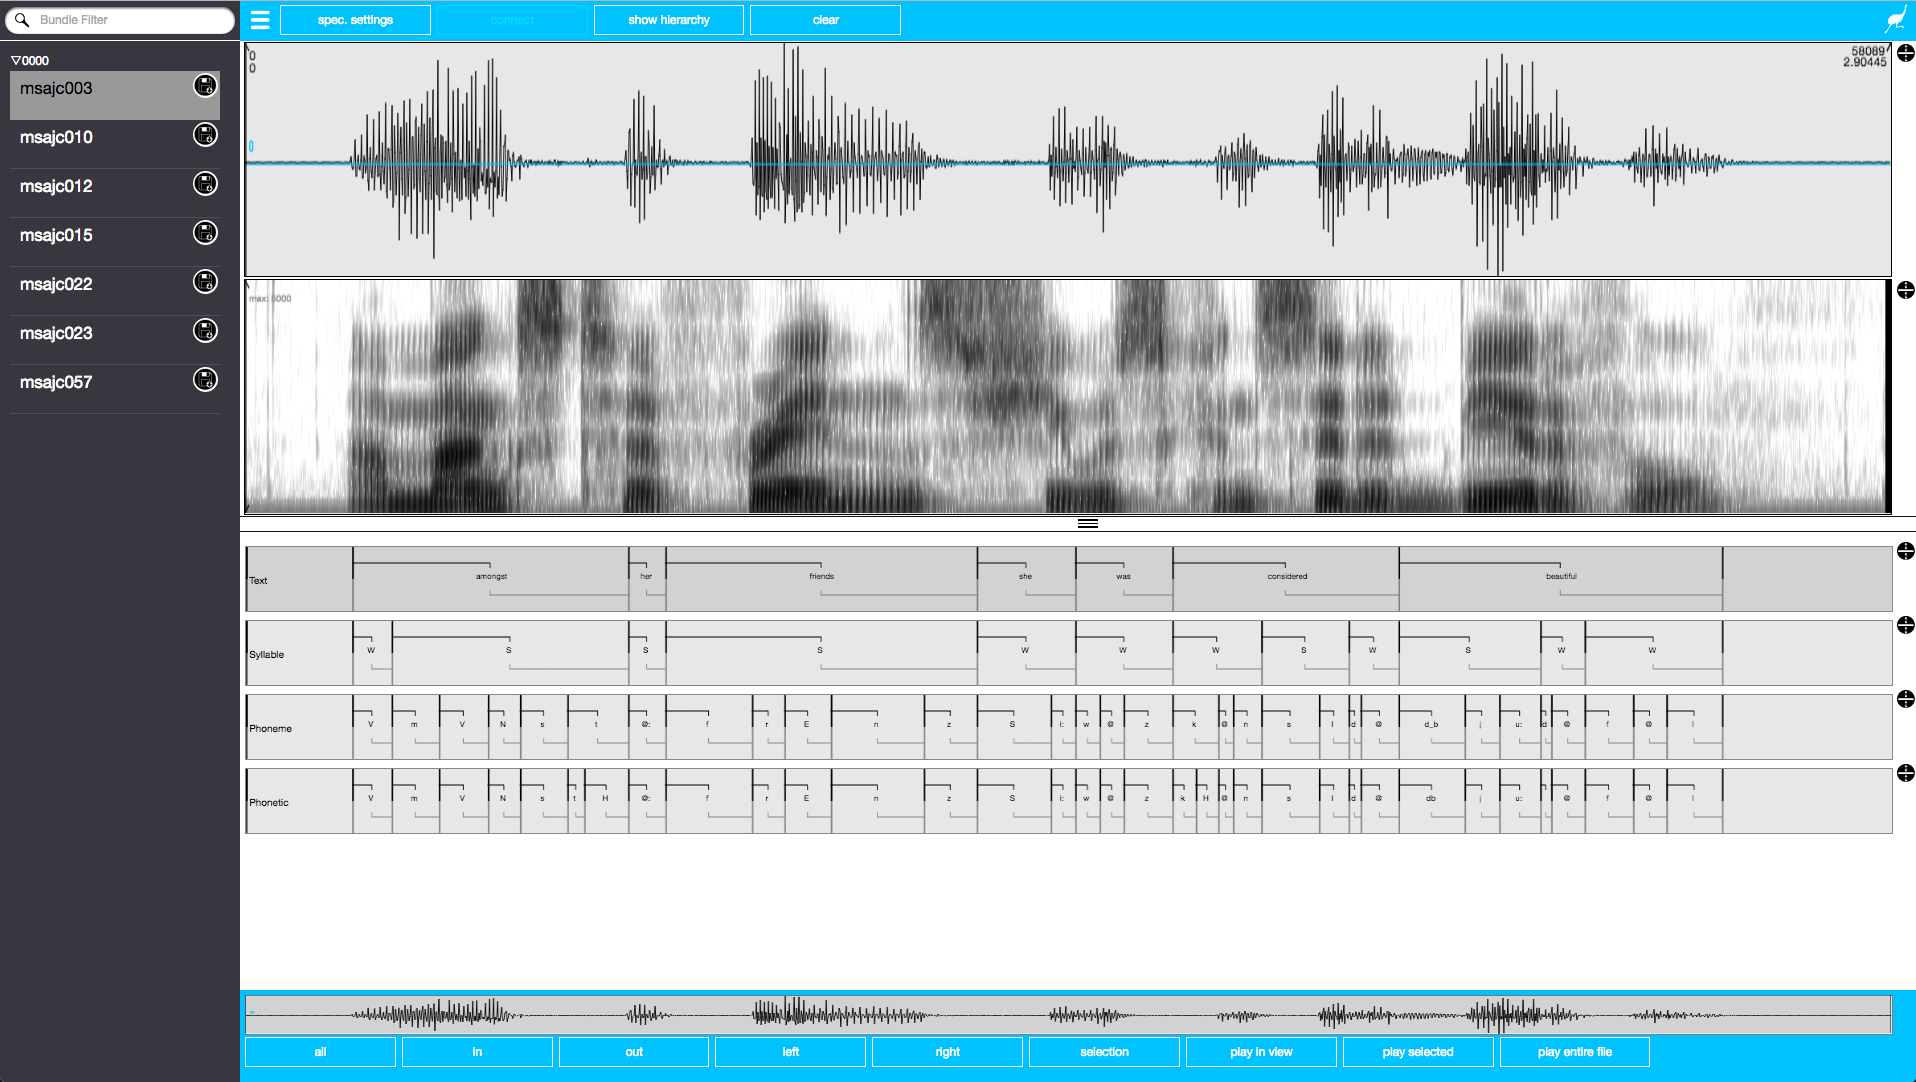
\includegraphics[width=1\linewidth]{pics/tutorialEmuWebAppMyFirst} 

}

\caption{Screenshot of `EMU-webApp` displaying `msajc003` bundle of *myFirst* `emuDB`.}\label{fig:tutorial-emuWebAppMyFirst}
\end{figure}

\hypertarget{querying-and-autobuilding-the-annotation-structure}{%
\subsection{Querying and autobuilding the annotation
structure}\label{querying-and-autobuilding-the-annotation-structure}}

An integral step in the default workflow of the EMU-SDMS is querying the
annotations of a database. The \texttt{emuR} package implements a
\texttt{query()} function to accomplish this task. This function
evaluates an EMU Query Language (EQL) expression and extracts the
annotation items from the database that match a query expression. As
Chapter \ref{chap:querysys} gives a detailed description of the query
mechanics provided by \texttt{emuR}, this tutorial will only use a very
small, hopefully easy to understand subset of the EQL.

The output of the \texttt{summary()} command in R Example
@ref(rexample:tutorial\_summary) and the screenshot in Figure
\ref{fig:tutorial-emuWebAppMyFirst} show that the \emph{myFirst}
\texttt{emuDB} contains four levels of annotations. R Example
\ref{rexample:tutorial-simpleQuery} shows four separate queries that
query various segments on each of the available levels. The query
expressions all use the matching operator \texttt{==} which returns
annotation items whose labels match those specified to the right of the
operator and that belong to the level specified to the left of the
operator (i.e., \texttt{LEVEL\ ==\ LABEL}; see Chapter
\ref{chap:querysys} for a detailed description).

rexample:tutorial-simpleQuery

\begin{Shaded}
\begin{Highlighting}[]
\CommentTok{# query all segments containing the label}
\CommentTok{# "C" (== content word) of the "Word" level}
\NormalTok{sl_text =}\StringTok{ }\KeywordTok{query}\NormalTok{(}\DataTypeTok{emuDBhandle =}\NormalTok{ dbHandle,}
                \DataTypeTok{query =} \StringTok{"Word == C"}\NormalTok{)}

\CommentTok{# query all segments containing the label}
\CommentTok{# "S" (== strong syllable) of the "Syllable" level}
\NormalTok{sl_syl =}\StringTok{ }\KeywordTok{query}\NormalTok{(}\DataTypeTok{emuDBhandle =}\NormalTok{ dbHandle,}
               \DataTypeTok{query =} \StringTok{"Syllable == S"}\NormalTok{)}

\CommentTok{# query all segments containing the label}
\CommentTok{# "f" on the "Phoneme" level}
\NormalTok{sl_phoneme =}\StringTok{ }\KeywordTok{query}\NormalTok{(dbHandle,}
                   \DataTypeTok{query =} \StringTok{"Phoneme == f"}\NormalTok{)}

\CommentTok{# query all segments containing the label}
\CommentTok{# "n" of the "Phonetic" level}
\NormalTok{sl_phonetic =}\StringTok{ }\KeywordTok{query}\NormalTok{(dbHandle,}
                    \DataTypeTok{query =} \StringTok{"Phonetic == n"}\NormalTok{)}

\CommentTok{# show class vector of query result}
\KeywordTok{class}\NormalTok{(sl_phonetic)}
\end{Highlighting}
\end{Shaded}

\begin{verbatim}
## [1] "emuRsegs"   "emusegs"    "data.frame"
\end{verbatim}

\begin{Shaded}
\begin{Highlighting}[]
\CommentTok{# show first entry of sl_phonetic}
\KeywordTok{head}\NormalTok{(sl_phonetic, }\DataTypeTok{n =} \DecValTok{1}\NormalTok{)}
\end{Highlighting}
\end{Shaded}

\begin{verbatim}
## segment  list from database:  myFirst 
## query was:  Phonetic == n 
##   labels    start      end session   bundle    level    type
## 1      n 1031.925 1195.925    0000 msajc003 Phonetic SEGMENT
\end{verbatim}

\begin{Shaded}
\begin{Highlighting}[]
\CommentTok{# show summary of sl_phonetic}
\KeywordTok{summary}\NormalTok{(sl_phonetic)}
\end{Highlighting}
\end{Shaded}

\begin{verbatim}
## segment  list from database:  myFirst 
## query was:  Phonetic == n 
##  with 12 segments
## 
## Segment distribution:
## 
##  n 
## 12
\end{verbatim}

As demonstrated in R Example @ref(rexample:tutorial\_simpleQuery), the
result of a query is an \texttt{emuRsegs} object, which is a super-class
of the common \texttt{data.frame}. This object is often referred to as a
segment list, or ``seglist''. A segment list carries information about
the extracted annotation items such as the extracted labels, the start
and end times of the segments, the sessions and bundles the items are
from and the levels they belong to. An in-depth description of the
information contained in a segment list is given in Section
\ref{sec:query-emuRsegs}. R Example @ref(rexample:tutorial\_simpleQuery)
shows that the \texttt{summary()} function can also be applied to a
segment list object to get an overview of what is contained within it.
This can be especially useful when dealing with larger segment lists.

\hypertarget{autobuilding}{%
\subsection{Autobuilding}\label{autobuilding}}

The simple queries illustrated above query segments from a single level
that match a certain label. However, the EMU-SDMS offers a mechanism for
performing inter-level queries such as: \emph{Query all Phonetic items
that contain the label ``n'' and are part of a content word}. For such
queries to be possible, the EMU-SDMS offers very sophisticated
annotation structure modeling capabilities, which are described in
Chapter \ref{chap:annot-struct-mod}. For the sake of this tutorial we
will focus on converting the flat segment level annotation structure
displayed in Figure \ref{fig:tutorial-emuWebAppMyFirst} to a
hierarchical form as displayed in Figure
\ref{fig:tutorial-violentlyHier}, where only the \emph{Phonetic} level
carries time information and the annotation items on the other levels
are explicitly linked to each other to form a hierarchical annotation
structure.

\begin{figure}
\centering
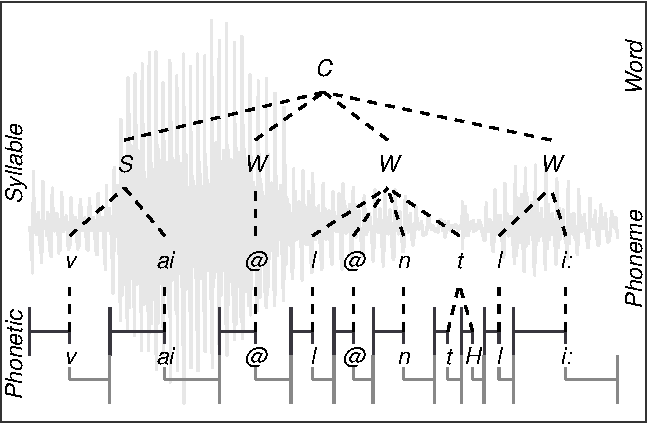
\includegraphics{tutorial_files/figure-latex/tutorial-violentlyHier-1.pdf}
\caption{\label{fig:tutorial-violentlyHier}Example of a hierarchical
annotation of the content (==\emph{C}) word \emph{violently} belonging
to the \emph{msajc012} bundle of the \emph{myFirst} demo
\texttt{emuDB}.}
\end{figure}

As it is a very laborious task to manually link annotation items
together using the \texttt{EMU-webApp} and the hierarchical information
is already implicitly contained in the time information of the segments
and events of each level, we will now use a function provided by the
\texttt{emuR} package to build these hierarchical structures using this
information called \texttt{autobuild\_linkFromTimes()}. R Example
\ref{rexample:tutorial-autobuild} shows the calls to this function which
autobuild the hierarchical annotations in the \emph{myFirst} database.
As a general rule for autobuilding hierarchical annotation structures, a
good strategy is to start the autobuilding process beginning with
coarser grained annotation levels (i.e., the \emph{Word}/\emph{Syllable}
level pair in our example) and work down to finer grained annotations
(i.e., the \emph{Syllable}/\emph{Phoneme} and
\emph{Phoneme}/\emph{Phonetic}\} level pairs in our example). To build
hierachical annotation structures we need link definitions, which
together with the level definitions define the annotation structure for
the entire database (see Chapter \ref{chap:annot-struct-mod} for further
details). The \texttt{autobuild\_linkFromTimes()} calls in R Example
\ref{rexample:tutorial-autobuild} use the \texttt{newLinkDefType}
parameter, which if defined automatically adds a link definition to the
database.

rexample:tutorial-autobuild

\begin{Shaded}
\begin{Highlighting}[]
\CommentTok{# invoke autobuild function}
\CommentTok{# for "Word" and "Syllable" levels}
\KeywordTok{autobuild_linkFromTimes}\NormalTok{(dbHandle,}
                        \DataTypeTok{superlevelName =} \StringTok{"Word"}\NormalTok{,}
                        \DataTypeTok{sublevelName =} \StringTok{"Syllable"}\NormalTok{,}
                        \DataTypeTok{convertSuperlevel =} \OtherTok{TRUE}\NormalTok{,}
                        \DataTypeTok{newLinkDefType =} \StringTok{"ONE_TO_MANY"}\NormalTok{)}

\CommentTok{# invoke autobuild function}
\CommentTok{# for "Syllable" and "Phoneme" levels}
\KeywordTok{autobuild_linkFromTimes}\NormalTok{(dbHandle,}
                        \DataTypeTok{superlevelName =} \StringTok{"Syllable"}\NormalTok{,}
                        \DataTypeTok{sublevelName =} \StringTok{"Phoneme"}\NormalTok{,}
                        \DataTypeTok{convertSuperlevel =} \OtherTok{TRUE}\NormalTok{,}
                        \DataTypeTok{newLinkDefType =} \StringTok{"ONE_TO_MANY"}\NormalTok{)}

\CommentTok{# invoke autobuild function}
\CommentTok{# for "Phoneme" and "Phonetic" levels}
\KeywordTok{autobuild_linkFromTimes}\NormalTok{(dbHandle,}
                        \DataTypeTok{superlevelName =} \StringTok{"Phoneme"}\NormalTok{,}
                        \DataTypeTok{sublevelName =} \StringTok{"Phonetic"}\NormalTok{,}
                        \DataTypeTok{convertSuperlevel =} \OtherTok{TRUE}\NormalTok{,}
                        \DataTypeTok{newLinkDefType =} \StringTok{"MANY_TO_MANY"}\NormalTok{)}
\end{Highlighting}
\end{Shaded}

\begin{figure}

{\centering 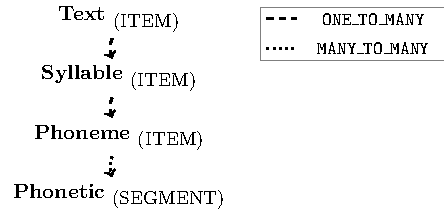
\includegraphics[width=0.5\linewidth]{pics/tut_simpleAnnotStruct} 

}

\caption{Schematic annotation structure of the `emuDB` after calling the autobuild function in R Example \ref{rexample:tutorial-autobuild}.}\label{fig:tutorial-simpleAnnotStruct}
\end{figure}

As the \texttt{autobuild\_linkFromTimes()} function automatically
creates backup levels to avoid the accidental loss of boundary or event
time information, R Example @ref(rexample:tutorial\_delBackupLevels)
shows how these backup levels can be removed to clean up the database.
However, using the \texttt{remove\_levelDefinition()} function with its
\texttt{force} parameter set to \texttt{TRUE} is a very invasive action.
Usually this would not be recommended, but for this tutorial we are
keeping everything as clean as possible.

rexample:tutorial-delBackupLevels

\begin{Shaded}
\begin{Highlighting}[]
\CommentTok{# list level definitions}
\CommentTok{# as this reveals the "-autobuildBackup" levels}
\CommentTok{# added by the autobuild_linkFromTimes() calls}
\KeywordTok{list_levelDefinitions}\NormalTok{(dbHandle)}
\end{Highlighting}
\end{Shaded}

\begin{verbatim}
##                       name    type nrOfAttrDefs              attrDefNames
## 1                     Word    ITEM            1                     Word;
## 2                 Syllable    ITEM            1                 Syllable;
## 3                  Phoneme    ITEM            1                  Phoneme;
## 4                 Phonetic SEGMENT            1                 Phonetic;
## 5     Word-autobuildBackup SEGMENT            1     Word-autobuildBackup;
## 6 Syllable-autobuildBackup SEGMENT            1 Syllable-autobuildBackup;
## 7  Phoneme-autobuildBackup SEGMENT            1  Phoneme-autobuildBackup;
\end{verbatim}

\begin{Shaded}
\begin{Highlighting}[]
\CommentTok{# remove the levels containing the "-autobuildBackup"}
\CommentTok{# suffix}
\KeywordTok{remove_levelDefinition}\NormalTok{(dbHandle,}
                       \DataTypeTok{name =} \StringTok{"Word-autobuildBackup"}\NormalTok{,}
                       \DataTypeTok{force =} \OtherTok{TRUE}\NormalTok{,}
                       \DataTypeTok{verbose =} \OtherTok{FALSE}\NormalTok{)}

\KeywordTok{remove_levelDefinition}\NormalTok{(dbHandle,}
                       \DataTypeTok{name =} \StringTok{"Syllable-autobuildBackup"}\NormalTok{,}
                       \DataTypeTok{force =} \OtherTok{TRUE}\NormalTok{,}
                       \DataTypeTok{verbose =} \OtherTok{FALSE}\NormalTok{)}

\KeywordTok{remove_levelDefinition}\NormalTok{(dbHandle,}
                       \DataTypeTok{name =} \StringTok{"Phoneme-autobuildBackup"}\NormalTok{,}
                       \DataTypeTok{force =} \OtherTok{TRUE}\NormalTok{,}
                       \DataTypeTok{verbose =} \OtherTok{FALSE}\NormalTok{)}

\CommentTok{# list level definitions}
\KeywordTok{list_levelDefinitions}\NormalTok{(dbHandle)}
\end{Highlighting}
\end{Shaded}

\begin{verbatim}
##       name    type nrOfAttrDefs attrDefNames
## 1     Word    ITEM            1        Word;
## 2 Syllable    ITEM            1    Syllable;
## 3  Phoneme    ITEM            1     Phoneme;
## 4 Phonetic SEGMENT            1    Phonetic;
\end{verbatim}

\begin{Shaded}
\begin{Highlighting}[]
\CommentTok{# list level definitions}
\CommentTok{# which were added by the autobuild functions}
\KeywordTok{list_linkDefinitions}\NormalTok{(dbHandle)}
\end{Highlighting}
\end{Shaded}

\begin{verbatim}
##           type superlevelName sublevelName
## 1  ONE_TO_MANY           Word     Syllable
## 2  ONE_TO_MANY       Syllable      Phoneme
## 3 MANY_TO_MANY        Phoneme     Phonetic
\end{verbatim}

As can be seen by the output of \texttt{list\_levelDefinitions()} and
\texttt{list\_linkDefinitions()} in R Example
\ref{rexample:tutorial-autobuild}, the annotation structure of the
\emph{myFirst} \texttt{emuDB} now matches that displayed in Figure
@ref(fig:tutorial\_simpleAnnotStruct). Using the \texttt{serve()}
function to open the \texttt{emuDB} in the \texttt{EMU-webApp} followed
by clicking on the \texttt{show\ hierarchy} button in the top menu (and
rotating the hierarchy by 90 degrees by clicking the
\texttt{rotate\ by\ 90\ degrees} button) will result in a view similar
to the screenshot of Figure
\ref{fig:tutorial-EMU-webAppScreenshotTutorialPostAutobHier}.

\begin{figure}

{\centering 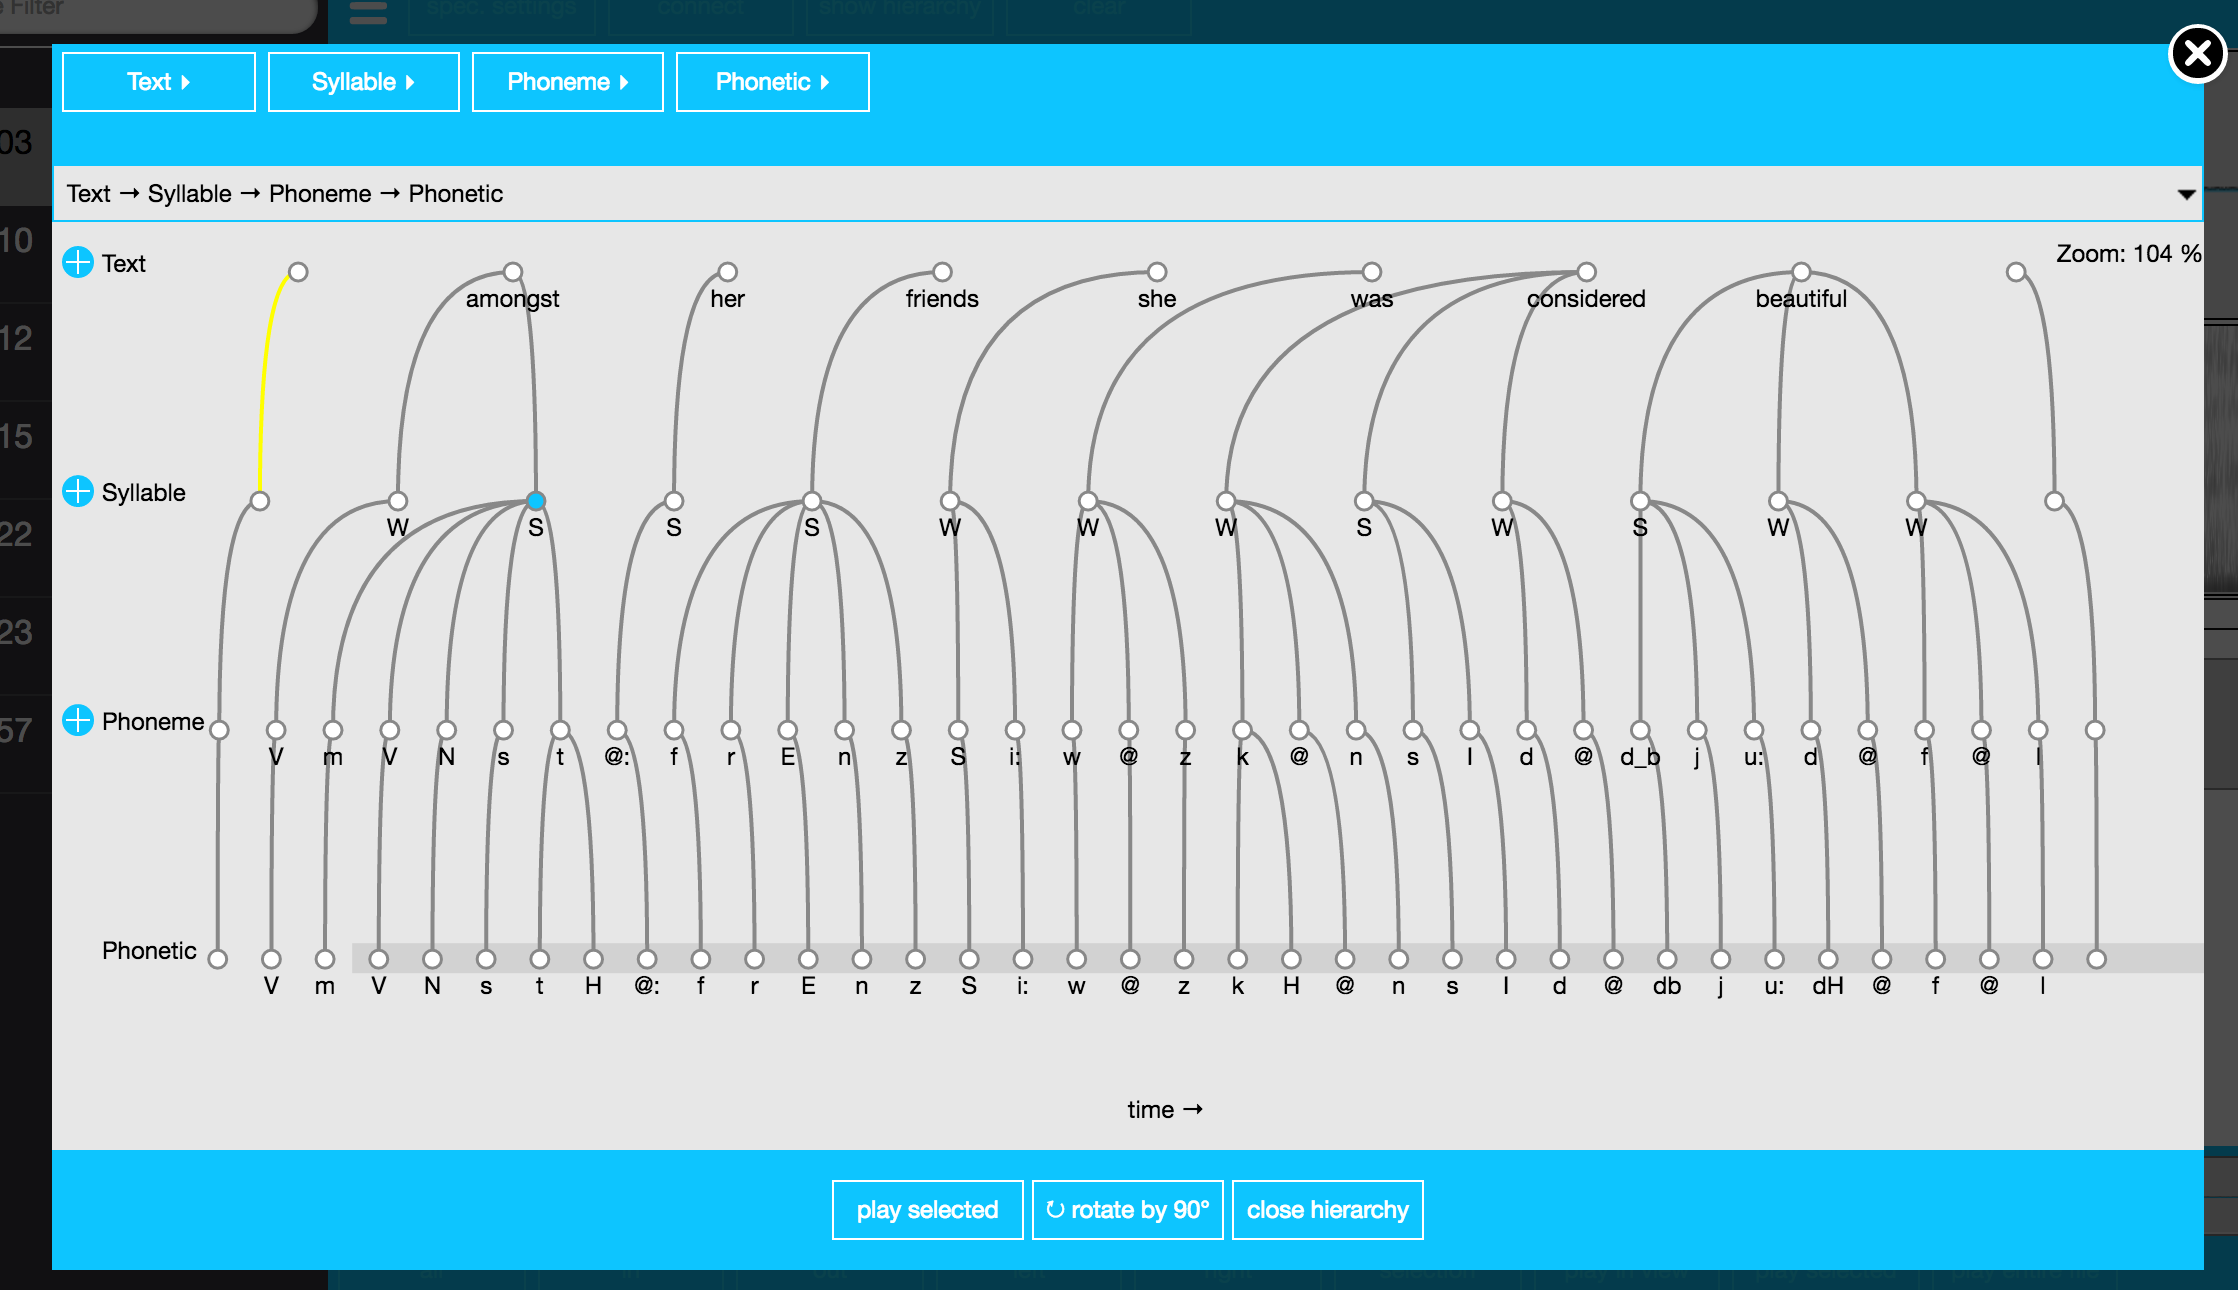
\includegraphics[width=1\linewidth]{pics/EMU-webAppScreenshotTutorialPostAutobHier} 

}

\caption{Screenshot of `EMU-webApp` displaying the autobuilt hierarchy of the *myFirst* `emuDB`.}\label{fig:webAppScreenshotTutorialPostAutobHier}
\end{figure}

\hypertarget{querying-the-hierarchical-annotations}{%
\subsubsection{Querying the hierarchical
annotations}\label{querying-the-hierarchical-annotations}}

Having this hierarchical annotation structure now allows us to formulate
a query that helps answer the originally stated question: \emph{Given an
annotated speech database, is the vowel height of the vowel @ (measured
by its correlate, the first formant frequency) influenced by whether it
appears in a content or function word?}. R Example
\ref{rexample:tutorial_labelGroupQuery} shows how all the
\emph{\citet{*} vowels in the }myFirst* database are queried.

rexample:tutorial-labelGroupQuery

\begin{Shaded}
\begin{Highlighting}[]
\CommentTok{# query annotation items containing}
\CommentTok{# the labels @ on the Phonetic level}
\NormalTok{sl_vowels =}\StringTok{ }\KeywordTok{query}\NormalTok{(dbHandle, }\StringTok{"Phonetic == @"}\NormalTok{)}

\CommentTok{# show first entry of sl_vowels}
\KeywordTok{head}\NormalTok{(sl_vowels, }\DataTypeTok{n =} \DecValTok{1}\NormalTok{)}
\end{Highlighting}
\end{Shaded}

\begin{verbatim}
## segment  list from database:  myFirst 
## query was:  Phonetic == @ 
##   labels    start      end session   bundle    level    type
## 1      @ 1506.175 1548.425    0000 msajc003 Phonetic SEGMENT
\end{verbatim}

As the type of word (content vs.~function) for each \emph{\citet{*}
vowel that was just extracted is also needed, we can use the requery
functionality of the EMU-SDMS (see Chapter \ref{chap:querysys}) to
retrieve the word type for each }@* vowel. A requery essentially moves
through a hierarchical annotation (vertically or horizontally) starting
from the segments that are passed into the requery function. R Example
\ref{rexample:tutorial-requery} illustrates the usage of the
hierarchical requery function, \texttt{requery\_hier()}, to retrieve the
appropriate annotation items from the *Word level.

rexample:tutorial-requery

\begin{Shaded}
\begin{Highlighting}[]
\CommentTok{# hierarchical requery starting from the items in sl_vowels}
\CommentTok{# and moving up to the "Word" level}
\NormalTok{sl_wordType =}\StringTok{ }\KeywordTok{requery_hier}\NormalTok{(dbHandle,}
                           \DataTypeTok{seglist =}\NormalTok{ sl_vowels,}
                           \DataTypeTok{level =} \StringTok{"Word"}\NormalTok{,}
                           \DataTypeTok{calcTimes =} \OtherTok{FALSE}\NormalTok{)}

\CommentTok{# show first entry of sl_wordType}
\KeywordTok{head}\NormalTok{(sl_wordType, }\DataTypeTok{n =} \DecValTok{1}\NormalTok{)}
\end{Highlighting}
\end{Shaded}

\begin{verbatim}
## segment  list from database:  myFirst 
## query was:  FROM REQUERY 
##   labels start end session   bundle level type
## 1      F    NA  NA    0000 msajc003  Word ITEM
\end{verbatim}

\begin{Shaded}
\begin{Highlighting}[]
\CommentTok{# show that sl_vowel and sl_wordType have the}
\CommentTok{# same number of row entries}
\KeywordTok{nrow}\NormalTok{(sl_vowels) }\OperatorTok{==}\StringTok{ }\KeywordTok{nrow}\NormalTok{(sl_wordType)}
\end{Highlighting}
\end{Shaded}

\begin{verbatim}
## [1] TRUE
\end{verbatim}

As can be seen by the \texttt{nrow()} comparison in R Example
\ref{rexample:tutorial-requery}, the segment list returned by the
\texttt{requery\_hier()} function has the same number of rows as the
original \texttt{sl\_vowels} segment list. This is important, as each
row of both segment lists line up and allow us to infer which segment
belongs to which word type (e.g., vowel \texttt{sl\_vowels{[}5,{]}}
belongs to the word type \texttt{sl\_wordType{[}5,{]}}).

\hypertarget{section:tutorial-sigExtrAndExpl}{%
\subsection{Signal extraction and
exploration}\label{section:tutorial-sigExtrAndExpl}}

Now that the vowel and word type information including the vowel start
and end time information has been extracted from the database, this
information can be used to extract signal data that matches these
segments. Using the \texttt{emuR} function \texttt{get\_trackdata()} we
can calculate the formant values in real time using the formant
estimation function, \texttt{forest()}, provided by the \texttt{wrassp}
package (see Chapter \ref{chap:wrassp} for details). R Example
\ref{rexample:tutorial-getTrackdata} shows the usage of this function.

rexample:tutorial-getTrackdata

\begin{Shaded}
\begin{Highlighting}[]
\CommentTok{# get formant values for the vowel segments}
\NormalTok{td_vowels =}\StringTok{ }\KeywordTok{get_trackdata}\NormalTok{(dbHandle,}
                          \DataTypeTok{seglist =}\NormalTok{ sl_vowels,}
                          \DataTypeTok{onTheFlyFunctionName =} \StringTok{"forest"}\NormalTok{,}
                          \DataTypeTok{verbose =}\NormalTok{ F)}

\CommentTok{# show class vector}
\KeywordTok{class}\NormalTok{(td_vowels)}
\end{Highlighting}
\end{Shaded}

\begin{verbatim}
## [1] "trackdata"
\end{verbatim}

\begin{Shaded}
\begin{Highlighting}[]
\CommentTok{# show dimensions}
\KeywordTok{dim}\NormalTok{(td_vowels)}
\end{Highlighting}
\end{Shaded}

\begin{verbatim}
## [1] 28  4
\end{verbatim}

\begin{Shaded}
\begin{Highlighting}[]
\CommentTok{# display all values for fifth segment}
\NormalTok{td_vowels[}\DecValTok{5}\NormalTok{,]}
\end{Highlighting}
\end{Shaded}

\begin{verbatim}
## trackdata from track: fm 
## index:
##  left right
##     1    12
## ftime:
##       start    end
## [1,] 2447.5 2502.5
## data:
##         T1   T2   T3   T4
## 2447.5 303 1031 2266 3366
## 2452.5 289  967 2250 3413
## 2457.5 296  905 2273 3503
## 2462.5 321  885 2357 3506
## 2467.5 316  889 2397 3475
## 2472.5 306  863 2348 3548
## 2477.5 314  832 2339 3611
## 2482.5 325  795 2342 3622
## 2487.5 339  760 2322 3681
## 2492.5 335  746 2316 3665
## 2497.5 341  734 2306 3688
## 2502.5 361  733 2304 3692
\end{verbatim}

As can be seen by the call to the \texttt{class()} function, the
resulting object is of the type \texttt{trackdata} and has 28 entries.
This corresponds to the number of rows contained in the segment lists
extracted above (i.e., \texttt{nrow(sl\_vowels)}). This indicates that
this object contains data for each of the segments that correspond to
each of the row entries of the segment lists (i.e.,
\texttt{td\_vowels{[}5,{]}} are the formant values belonging to
\texttt{sl\_vowels{[}5,{]}}). As the columns \texttt{T1}, \texttt{T2},
\texttt{T3}, \texttt{T4} of the printed output of
\texttt{td\_vowels{[}5,{]}} suggest, the \texttt{forest} function
estimates four formant values. We will only be concerned with the first
(column \texttt{T1}) and second (column \texttt{T2}). R Example
\ref{rexample:tutorial-dplot} shows a call to \texttt{emuR}'s
\texttt{dplot()} function which produces the plot displayed in Figure
\ref{fig:tutorial-dplot}. The first call to the \texttt{dplot()}
function plots all 28 first formant trajectories (achieved by indexing
the first column i.e., \texttt{T1}:
\texttt{x\ =\ td\_vowels{[},\ 1{]}}). To clean up the cluttered left
plot, the second call to the \texttt{dplot()} function additionally uses
the \texttt{average} parameter to plot only the ensemble averages of all
*\citet{*} vowels and time-normalizes the trajectories
(\texttt{normalise\ =\ TRUE}) to an interval between 0 and 1.

rexample:tutorial-dplot

\begin{Shaded}
\begin{Highlighting}[]
\CommentTok{# two plots next to each other}
\NormalTok{formantNr =}\StringTok{ }\DecValTok{1}

\KeywordTok{par}\NormalTok{(}\DataTypeTok{mfrow =} \KeywordTok{c}\NormalTok{(}\DecValTok{1}\NormalTok{,}\DecValTok{2}\NormalTok{))}

\KeywordTok{dplot}\NormalTok{(}\DataTypeTok{x =}\NormalTok{ td_vowels[, formantNr],}
      \DataTypeTok{labs =}\NormalTok{ sl_vowels}\OperatorTok{$}\NormalTok{labels,}
      \DataTypeTok{xlab =} \StringTok{"Duration (ms)"}\NormalTok{,}
      \DataTypeTok{ylab =} \KeywordTok{paste0}\NormalTok{(}\StringTok{"F"}\NormalTok{, formantNr, }\StringTok{" (Hz)"}\NormalTok{))}

\KeywordTok{dplot}\NormalTok{(}\DataTypeTok{x =}\NormalTok{ td_vowels[, }\DecValTok{1}\NormalTok{],}
      \DataTypeTok{labs =}\NormalTok{ sl_vowels}\OperatorTok{$}\NormalTok{labels,}
      \DataTypeTok{normalise =} \OtherTok{TRUE}\NormalTok{,}
      \DataTypeTok{average =} \OtherTok{TRUE}\NormalTok{,}
      \DataTypeTok{xlab =} \StringTok{"Normalized time"}\NormalTok{,}
      \DataTypeTok{ylab =} \KeywordTok{paste0}\NormalTok{(}\StringTok{"F"}\NormalTok{, formantNr, }\StringTok{" (Hz)"}\NormalTok{))}

\CommentTok{# back to single plot}
\KeywordTok{par}\NormalTok{(}\DataTypeTok{mfrow =} \KeywordTok{c}\NormalTok{(}\DecValTok{1}\NormalTok{,}\DecValTok{1}\NormalTok{))}
\end{Highlighting}
\end{Shaded}

\begin{figure}
\centering
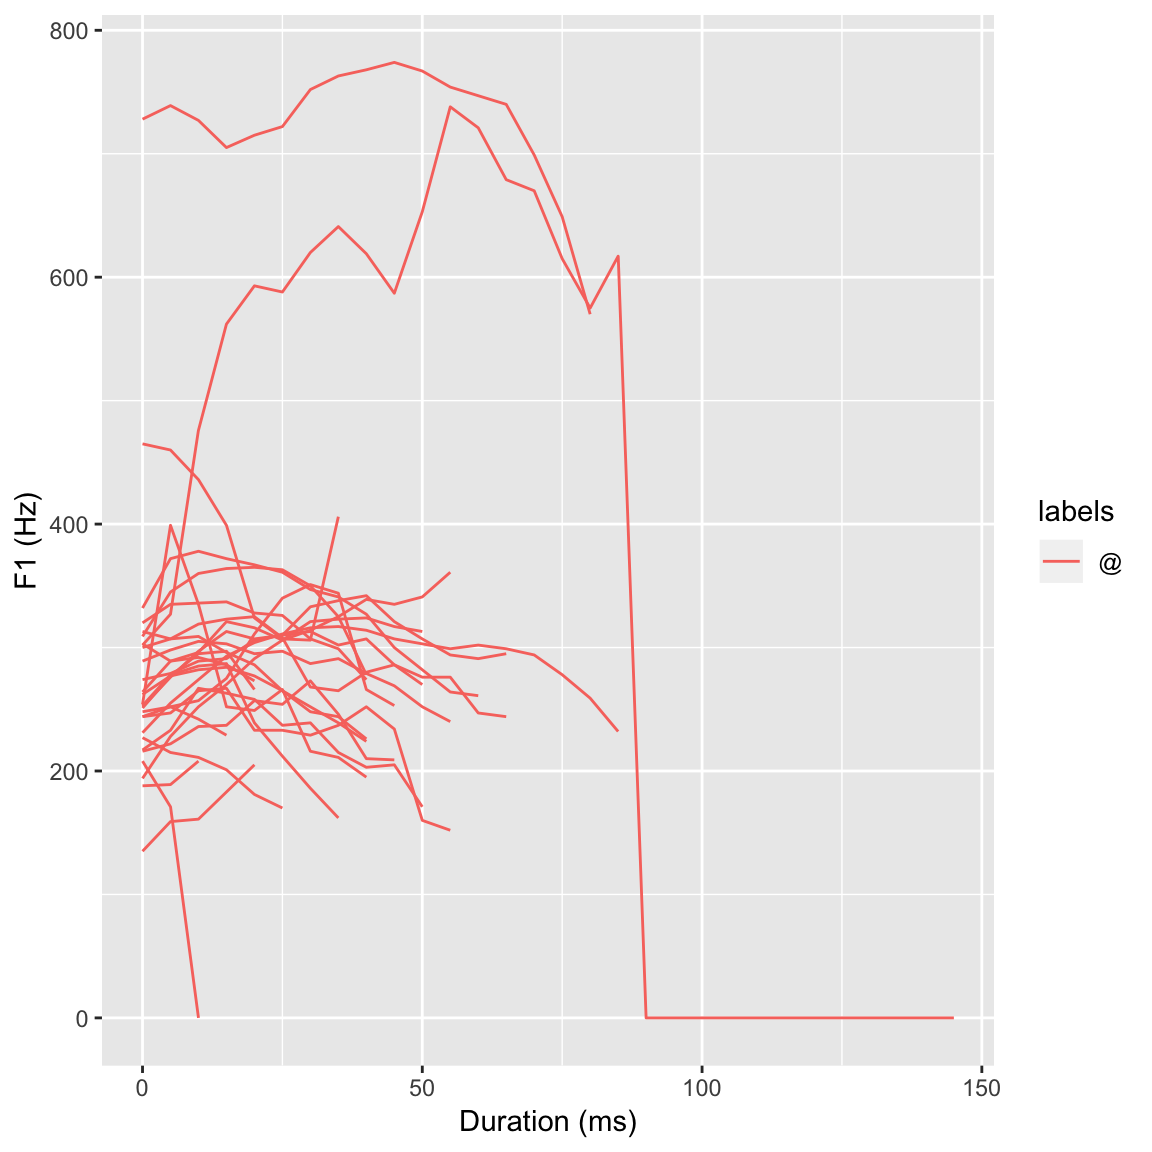
\includegraphics{tutorial_files/figure-latex/tutorial-dplot-1.pdf}
\caption{\label{fig:tutorial-dplot}\texttt{dplot()} plots of F1
trajectories. The left plot displays all trajectories while the right
plot displays the ensemble average of all *\citet{*} vowels.}
\end{figure}

Figure \ref{fig:tutorial-dplot} gives an overview of the first formant
trajectories of the *\citet{*} vowels. For the purpose of data
exploration and to get an idea of where the individual vowel classes lie
on the F2 x F1 plane, which indirectly provides information about vowel
height and tongue position, R Example \ref{rexample:tutorial-eplot}
makes use of the \texttt{eplot()} function. This produces Figure
\ref{fig:tutorial-eplot}. To be able to use the \texttt{eplot()}
function, the \texttt{td\_vowels} object first has to be modified, as it
contains entire formant trajectories but two dimensional data is needed
to be able to display it on the F2 x F1 plain. This can, for example, be
achieved by only extracting temporal mid-point formant values for each
vowel using the \texttt{get\_trackdata()} function utilizing its
\texttt{cut} parameter. R Example \ref{rexample:tutorial-eplot} shows an
alternative approach using the \texttt{dcut()} function to essentially
cut the formant trajectories to a specified proportional segment. By
using only the \texttt{left.time\ =\ 0.5} (and not specifying
\texttt{right.time}) only the formant values that are closest to the
temporal mid-point are cut from the trajectories.

rexample:tutorial-eplot

\begin{Shaded}
\begin{Highlighting}[]
\CommentTok{# cut formant trajectories at temporal mid-point}
\NormalTok{td_vowels_midpoint =}\StringTok{ }\KeywordTok{dcut}\NormalTok{(td_vowels,}
                          \DataTypeTok{left.time =} \FloatTok{0.5}\NormalTok{,}
                          \DataTypeTok{prop =} \OtherTok{TRUE}\NormalTok{)}

\CommentTok{# show dimensions of td_vowels_midpoint}
\KeywordTok{dim}\NormalTok{(td_vowels_midpoint)}

\CommentTok{# generate plot}
\KeywordTok{eplot}\NormalTok{(}\DataTypeTok{x =}\NormalTok{ td_vowels_midpoint[,}\DecValTok{1}\OperatorTok{:}\DecValTok{2}\NormalTok{],}
      \DataTypeTok{labs =}\NormalTok{ sl_vowels}\OperatorTok{$}\NormalTok{labels,}
      \DataTypeTok{dopoints =} \OtherTok{TRUE}\NormalTok{,}
      \DataTypeTok{formant =} \OtherTok{TRUE}\NormalTok{,}
      \DataTypeTok{xlab=}\StringTok{"F2 (Hz)"}\NormalTok{,}
      \DataTypeTok{ylab =} \StringTok{"F1 (Hz)"}
\NormalTok{      )}
\end{Highlighting}
\end{Shaded}

\begin{figure}
\centering
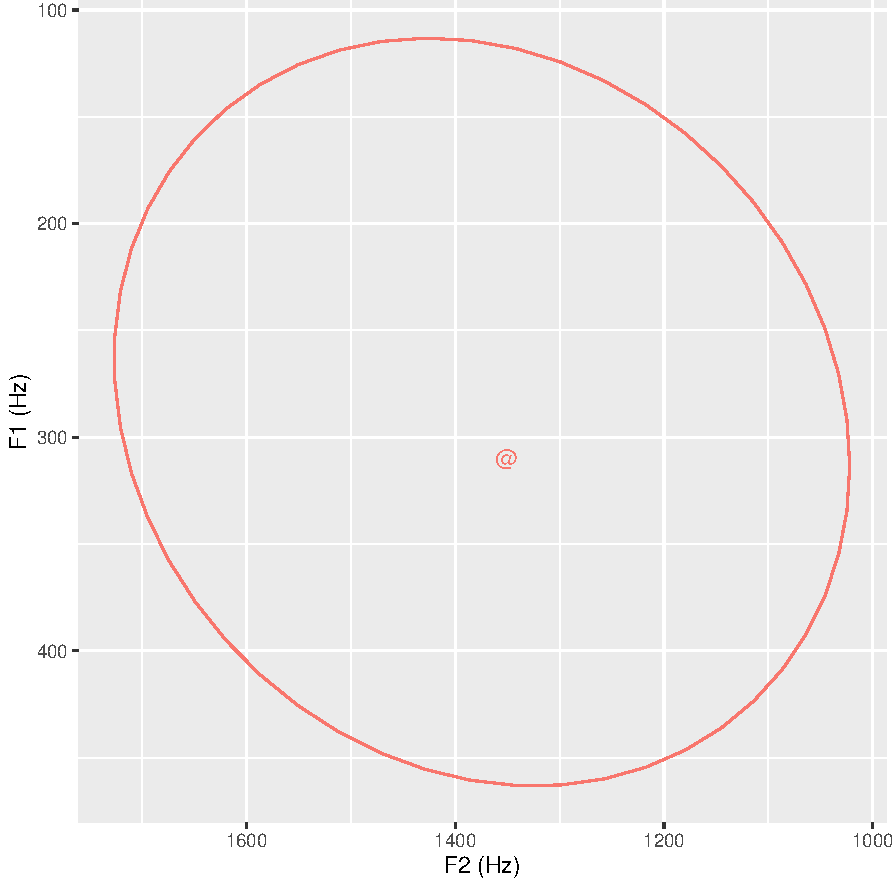
\includegraphics{tutorial_files/figure-latex/tutorial-eplot-1.pdf}
\caption{\label{fig:tutorial-eplot}95\% ellipses for F2 x F1 data extracted
from the temporal midpoint of the vowel segments.}
\end{figure}

Figure @ref\{fig:tutorial-eplot\} displays the first two formants
extracted at the temporal midpoint of every *\citet{*} vowel in
\texttt{sl\_vowels}. These formants are plotted on the F2 x F1 plane,
and their 95\% ellipsis distribution is also shown. Although not
necessarily applicable to the question posed at the beginning of this
tutorial, the data exploration using the \texttt{dplot()} and
\texttt{eplot()} functions can be very helpful tools for providing an
overview of the data at hand.

\hypertarget{vowel-height-as-a-function-of-word-types-content-vs.function-evaluation-and-statistical-analysis}{%
\subsection{Vowel height as a function of word types (content
vs.~function): evaluation and statistical
analysis}\label{vowel-height-as-a-function-of-word-types-content-vs.function-evaluation-and-statistical-analysis}}

The above data exploration only dealt with the actual \emph{\citet{*}
vowels and disregarded the syllable type they occurred in. However, the
question in the introduction of this chapter focuses on whether the }@*
vowel occurs in a content (labeled \emph{C}) or function (labeled
\emph{F}) word. For data inspection purposes, R Example
\ref{rexample:tutorial-dplotSylTyp} initially extracts the central 60\%
(\texttt{left.time\ =\ 0.2} and \texttt{right.time\ =\ 0.8}) of the
formant trajectories from \texttt{td\_vowels} using \texttt{dcut()} and
displays them using \texttt{dplot()}. It should be noted that the call
to \texttt{dplot()} uses the labels of the \texttt{sl\_wordType} object
as opposed to those of \texttt{sl\_vowels}. This causes the
\texttt{dplot()} functions to group the trajectories by their word type
as opposed to their vowel labels as displayed in Figure
@ref(fig:tutorial\_dplotSylTyp).

rexample:tutorial-dplotSylTyp

\begin{Shaded}
\begin{Highlighting}[]
\CommentTok{# extract central 60% from formant trajectories}
\NormalTok{td_vowelsMidSec =}\StringTok{ }\KeywordTok{dcut}\NormalTok{(td_vowels,}
                       \DataTypeTok{left.time =} \FloatTok{0.2}\NormalTok{,}
                       \DataTypeTok{right.time =} \FloatTok{0.8}\NormalTok{,}
                       \DataTypeTok{prop =} \OtherTok{TRUE}\NormalTok{)}

\CommentTok{# plot first formant trajectories}
\NormalTok{formantNr =}\StringTok{ }\DecValTok{1}
\KeywordTok{dplot}\NormalTok{(}\DataTypeTok{x =}\NormalTok{ td_vowelsMidSec[, formantNr],}
      \DataTypeTok{labs =}\NormalTok{ sl_wordType}\OperatorTok{$}\NormalTok{labels,}
      \DataTypeTok{normalise =} \OtherTok{TRUE}\NormalTok{,}
      \DataTypeTok{average =} \OtherTok{TRUE}\NormalTok{,}
      \DataTypeTok{xlab =} \StringTok{"Normalized time"}\NormalTok{,}
      \DataTypeTok{ylab =} \KeywordTok{paste}\NormalTok{(}\StringTok{"F"}\NormalTok{, formantNr, }\StringTok{" (Hz)"}\NormalTok{))}
\end{Highlighting}
\end{Shaded}

\begin{figure}
\centering
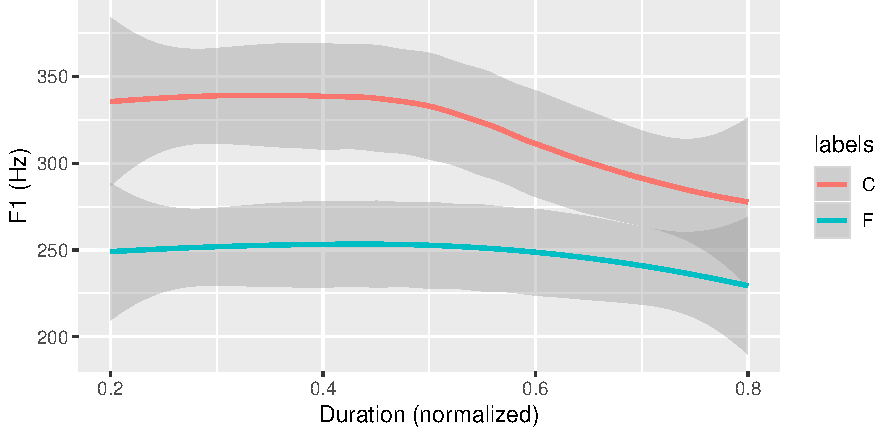
\includegraphics{tutorial_files/figure-latex/tutorial-dplotSylTyp-1.pdf}
\caption{\label{fig:tutorial-dplotSylTyp}Ensemble averages of F1 contours of
all tokens of the central 60\% of vowels grouped by word type (function
(\emph{F}) vs.~content (\emph{W})).}
\end{figure}

As can be seen in Figure \ref{fig:tutorial-dplotSylTyp}, there seems to
be a distinction in F1 trajectory height between vowels in content and
function words. R Example \ref{rexample:tutorial-boxplot} shows the code
to produce a boxplot using the \texttt{ggplot2} package to further
visually inspect the data (see Figure \ref{fig:tutorial-boxplot} for the
plot produced by R Example @ref\{rexample:tutorial-boxplot\}).

rexample:tutorial-boxplot

\begin{Shaded}
\begin{Highlighting}[]
\NormalTok{formantNr =}\StringTok{ }\DecValTok{1}
\CommentTok{# use trapply to calculate the means of the 60%}
\CommentTok{# formant trajectories}
\NormalTok{td_vowelsMidSec_mean =}\StringTok{ }\KeywordTok{trapply}\NormalTok{(td_vowelsMidSec[, formantNr],}
                               \DataTypeTok{fun =}\NormalTok{ mean,}
                               \DataTypeTok{simplify =}\NormalTok{ T)}

\CommentTok{# create new data frame that contains the mean}
\CommentTok{# values and the corresponding labels}
\NormalTok{df =}\StringTok{ }\KeywordTok{data.frame}\NormalTok{(}\DataTypeTok{wordType =}\NormalTok{ sl_wordType}\OperatorTok{$}\NormalTok{labels,}
                \DataTypeTok{meanF1 =}\NormalTok{ td_vowelsMidSec_mean)}

\CommentTok{# load library}
\KeywordTok{library}\NormalTok{(ggplot2)}

\CommentTok{# create boxplot using ggplot}
\KeywordTok{ggplot}\NormalTok{(df, }\KeywordTok{aes}\NormalTok{(wordType, meanF1)) }\OperatorTok{+}
\StringTok{  }\KeywordTok{geom_boxplot}\NormalTok{() }\OperatorTok{+}
\StringTok{  }\KeywordTok{labs}\NormalTok{(}\DataTypeTok{x =} \StringTok{"Word type"}\NormalTok{, }\DataTypeTok{y =} \KeywordTok{paste0}\NormalTok{(}\StringTok{"mean F"}\NormalTok{, formantNr, }\StringTok{" (Hz)"}\NormalTok{))}
\end{Highlighting}
\end{Shaded}

\begin{figure}
\centering
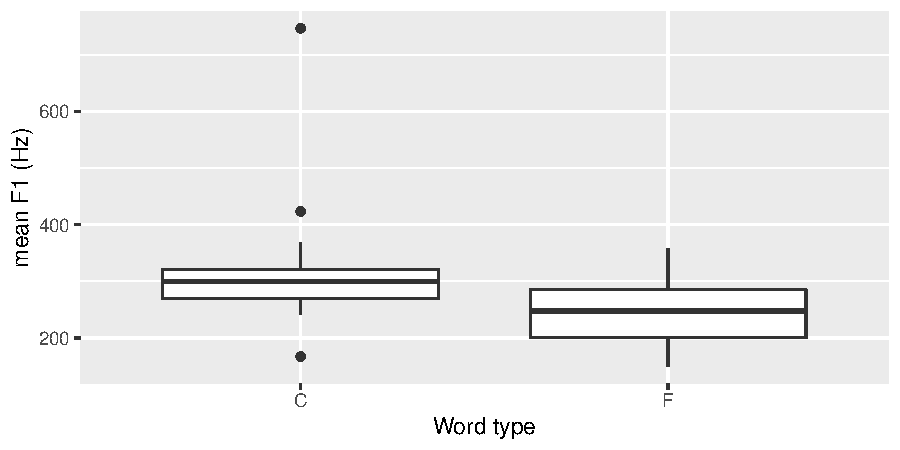
\includegraphics{tutorial_files/figure-latex/tutorial-boxplot-1.pdf}
\caption{\label{fig:tutorial-boxplot}Boxplot produced using \texttt{ggplot2}
to visualize the difference in F1 depending on whether the vowel occurs
in content (\emph{C}) or function (\emph{F}) word.}
\end{figure}

To confirm or reject this, R Example \ref{rexample:tutorial-stats1}
presents a very simple statistical analysis of the F1 mean values of the
60\% mid-section formant trajectories \footnote{It is worth noting that
  the sample size in this toy example is quite small. This obviously
  influences the outcome of the simple statistical analysis that is
  performed here.}. First, a Shapiro-Wilk test for normality of the
distributions of the F1 means for both word types is carried out. As
only one type is normally distributed, a Wilcoxon rank sum test is
performed. The density distributions (commented out \texttt{plot()}
function calls in R Example \ref{rexample:tutorial-stats1}) are
displayed in Figure @ref(fig:tutorial\_stats1).

rexample:tutorial-stats1

\begin{Shaded}
\begin{Highlighting}[]
\CommentTok{# calculate density for vowels in function words}
\NormalTok{distrF =}\StringTok{ }\KeywordTok{density}\NormalTok{(df[df}\OperatorTok{$}\NormalTok{wordType }\OperatorTok{==}\StringTok{ "F"}\NormalTok{,]}\OperatorTok{$}\NormalTok{meanF1)}

\CommentTok{# uncomment to visualize distribution}
\CommentTok{# plot(distrF)}

\CommentTok{# check that vowels in function}
\CommentTok{# words are normally distributed}
\KeywordTok{shapiro.test}\NormalTok{(df[df}\OperatorTok{$}\NormalTok{wordType }\OperatorTok{==}\StringTok{ "F"}\NormalTok{,]}\OperatorTok{$}\NormalTok{meanF1)}
\end{Highlighting}
\end{Shaded}

\begin{verbatim}
## 
##  Shapiro-Wilk normality test
## 
## data:  df[df$wordType == "F", ]$meanF1
## W = 0.98687, p-value = 0.9887
\end{verbatim}

\begin{Shaded}
\begin{Highlighting}[]
\CommentTok{# p-value > 0.05 implying that the distribution}
\CommentTok{# of the data ARE NOT significantly different from}
\CommentTok{# normal distribution -> we CAN assume normality}

\CommentTok{# calculate density for vowels in content words}
\NormalTok{distrC =}\StringTok{ }\KeywordTok{density}\NormalTok{(df[df}\OperatorTok{$}\NormalTok{wordType }\OperatorTok{==}\StringTok{ "C"}\NormalTok{,]}\OperatorTok{$}\NormalTok{meanF1)}

\CommentTok{# uncomment to visualize distribution}
\CommentTok{# plot(distrC)}

\CommentTok{# check that vowels in content}
\CommentTok{# words are normally distributed:}
\KeywordTok{shapiro.test}\NormalTok{(df[df}\OperatorTok{$}\NormalTok{wordType }\OperatorTok{==}\StringTok{ "C"}\NormalTok{,]}\OperatorTok{$}\NormalTok{meanF1)}
\end{Highlighting}
\end{Shaded}

\begin{verbatim}
## 
##  Shapiro-Wilk normality test
## 
## data:  df[df$wordType == "C", ]$meanF1
## W = 0.66506, p-value = 1.506e-05
\end{verbatim}

\begin{Shaded}
\begin{Highlighting}[]
\CommentTok{# p-value < 0.05 implying that the distribution}
\CommentTok{# of the data ARE significantly different from}
\CommentTok{# normal distribution -> we CAN NOT assume normality}
\CommentTok{# (this somewhat unexpected result is probably}
\CommentTok{# due to the small sample size used in this toy example)}
\CommentTok{# -> use Wilcoxon rank sum test}

\CommentTok{# perform Wilcoxon rank sum test to establish}
\CommentTok{# whether vowel F1 depends on word type}
\KeywordTok{wilcox.test}\NormalTok{(meanF1 }\OperatorTok{~}\StringTok{ }\NormalTok{wordType, }\DataTypeTok{data =}\NormalTok{ df)}
\end{Highlighting}
\end{Shaded}

\begin{verbatim}
## 
##  Wilcoxon rank sum test
## 
## data:  meanF1 by wordType
## W = 121, p-value = 0.03752
## alternative hypothesis: true location shift is not equal to 0
\end{verbatim}

\begin{figure}
\centering
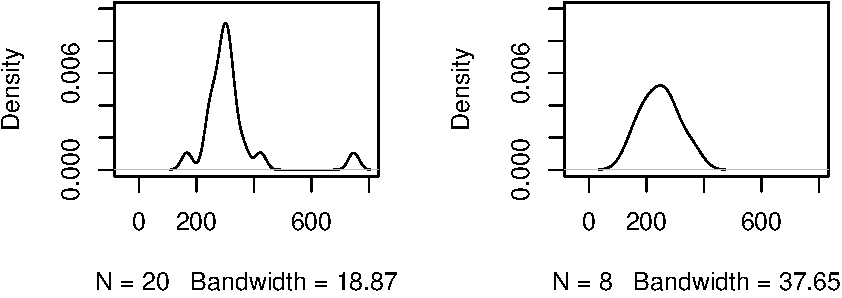
\includegraphics{tutorial_files/figure-latex/tutorial-stats1-1.pdf}
\caption{\label{fig:tutorial-stats1}Plots of density distributions of vowels
in content words (left plot) and vowels in function words (right plot)
in R Example \citet{ref}(rexample:tutorial\_stats1).}
\end{figure}

As shown by the result of \texttt{wilcox.test()} in R Example
@ref(rexample:tutorial\_stats1), word type (\emph{C} vs. \emph{F}) has a
significant influence on the vowel's F1 (W=121, p\textless{}0.05).
Hence, the answer to the initially proposed question: \emph{Given an
annotated speech database, is vowel height of the vowel @ (measured by
its correlate, the first formant frequency) influenced by whether it
appears in a content or function word?} is yes!

\hypertarget{conclusion}{%
\subsection{Conclusion}\label{conclusion}}

The tutorial given in this chapter gave an overview of what it is like
working with the EMU-SDMS to try to solve a research question. As many
of the concepts were only briefly explained, it is worth noting that
explicit explanations of the various components and integral concepts
are given in following chapters. Further, additional use cases that have
been taken from the \texttt{emuR\_intro} vignette can be found in
Appendix @ref(app\_chap:useCases). These use cases act as templates for
various types of research questions and will hopefully aid the user in
finding a solution similar to what she or he wishes to achieve.


\end{document}
